\chapter{Diseño de clases} \label{cap:diseño_clases}

\section{Introducción}

En este capítulo se realizará una breve introducción sobre el diagrama de clases y posteriormente, un análisis de las clases que participan en el modelo de información del simulador SimAS 3.0. Para ello, se especificarán los atributos, métodos y las relaciones existentes entre las mismas, terminándose con un diagrama de clases general de todo el sistema.

El propósito de un diagrama de clases es el de representar los objetos fundamentales del sistema, es decir, los que percibe el usuario y con los que espera tratar para completar su tarea. Una clase define el ámbito de definición de un conjunto de objetos.

Cada clase se representa en un rectángulo con tres apartados:
\begin{itemize}
\item Nombre de la clase.
\item Atributos de la clase.
\item Operaciones de la clase.
\end{itemize}

En SimAS 3.0, el diseño de clases sigue el patrón Model-View-Controller (MVC), donde las clases del modelo representan la lógica de negocio y los datos de las gramáticas de contexto libre, mientras que las clases de la vista y controlador manejan la interfaz de usuario y la interacción con el usuario.


\section{Diseño de clases por paquetes}

El sistema SimAS 3.0 está organizado en 8 paquetes principales que contienen un total de 51 clases Java. Para una mejor comprensión y organización, este capítulo presenta las clases agrupadas por paquetes, siguiendo la arquitectura por capas definida en el Capítulo 8.

Cada sección dedicada a un paquete incluye:
\begin{itemize}
    \item \textbf{Introducción}: propósito y responsabilidad del paquete.
    \item \textbf{Clases principales}: análisis detallado de cada clase con atributos y métodos.
    \item \textbf{Dependencias internas}: relaciones entre clases dentro del paquete.
    \item \textbf{Patrones de diseño}: patrones utilizados en el paquete.
\end{itemize}

\subsection{Paquete bienvenida}

El paquete \textbf{bienvenida} contiene las clases responsables de la inicialización y navegación principal de la aplicación SimAS 3.0. Este paquete implementa el patrón Singleton y Facade para gestionar el ciclo de vida de la aplicación.

\subsubsection{Clases del paquete bienvenida}

Este paquete contiene 2 clases principales que gestionan el punto de entrada y la navegación inicial del sistema.

\subsubsection{Clase Bienvenida}

Esta clase representa la pantalla de bienvenida de la aplicación SimAS 3.0, heredando de Application para ser el punto de entrada principal.

\begin{longtable}[H]{|>{\columncolor[rgb]{0.63,0.79,0.95}}m{6cm} | m{8.5cm} |}
 \caption{Clase Bienvenida}

\endfirsthead

\multicolumn{2}{c}
{{\tablename\ \thetable{} -- continúa de la página anterior}} \\
\endhead

\hline \multicolumn{2}{|r|}{{Continúa en la página siguiente}} \\ \hline
\endfoot

\hline
\endlastfoot

\hline
 \textbf{Nombre} & \textbf{Bienvenida}  \\ \hline
 
 \textbf{Descripción} & Representa la pantalla de bienvenida de la aplicación.  \\ \hline
                       
 \textbf{Atributos} & \begin{enumerate}
 		\item \textbf{stage}: Stage principal de la aplicación JavaFX.
 		\item \textbf{scene}: Scene que contiene la interfaz de bienvenida.
 		\item \textbf{root}: VBox principal que organiza el layout vertical.
 		\item \textbf{logo}: ImageView que muestra el logo de la aplicación.
 		\item \textbf{titulo}: Label con el título principal de SimAS 3.0.
 		\item \textbf{subtitulo}: Label con información adicional.
 		\item \textbf{selectorIdioma}: ComboBox para selección de idioma.
 		\item \textbf{botonContinuar}: Button para acceder al menú principal.
 		\item \textbf{bundle}: ResourceBundle para internacionalización.
 		\item \textbf{idiomaSeleccionado}: String con el código del idioma actual.
 		\item \textbf{preferencias}: Properties para guardar configuración.
 		\item \textbf{animacionFadeIn}: FadeTransition para animación de entrada.
 		\item \textbf{timeline}: Timeline para animaciones secuenciales.
 		\item \textbf{esPrimeraEjecucion}: boolean que indica si es la primera vez.
 		\item \textbf{versionAplicacion}: String con la versión actual.
 		\item \textbf{fechaCompilacion}: String con la fecha de compilación.
\end{enumerate} \\ \hline
 
\textbf{Métodos} & \begin{enumerate}
 		\item \textbf{start(Stage)}: método principal que inicializa la aplicación y configura la escena inicial.
 		\item \textbf{main(String[])}: punto de entrada estático de la aplicación JavaFX.
 		\item \textbf{inicializarInterfaz()}: configura todos los elementos visuales de la pantalla de bienvenida.
 		\item \textbf{configurarIdioma()}: detecta y configura el idioma por defecto del sistema.
 		\item \textbf{cargarRecursos()}: carga imágenes, estilos y recursos necesarios.
 		\item \textbf{crearLayoutPrincipal()}: crea el layout principal con VBox y elementos centrados.
 		\item \textbf{agregarLogo()}: añade el logo de la aplicación al centro.
 		\item \textbf{agregarTitulo()}: añade el título principal de la aplicación.
 		\item \textbf{agregarSelectorIdioma()}: crea el ComboBox para selección de idioma.
 		\item \textbf{agregarBotonContinuar()}: añade el botón para continuar al menú principal.
 		\item \textbf{configurarEstilos()}: aplica estilos CSS a todos los componentes.
 		\item \textbf{animarEntrada()}: ejecuta animaciones de entrada suaves.
 		\item \textbf{transitarAMenuPrincipal()}: realiza la transición suave al menú principal.
 		\item \textbf{guardarPreferenciasIdioma()}: guarda la selección de idioma del usuario.
 		\item \textbf{cargarPreferencias()}: carga preferencias guardadas anteriormente.
\end{enumerate} \\ \hline

\textbf{Métodos} & \begin{enumerate}
 		\item \textbf{verificarPrimeraEjecucion()}: determina si es la primera vez que se ejecuta.
 		\item \textbf{mostrarTutorialInicial()}: muestra tutorial básico para nuevos usuarios.
 		\item \textbf{centrarVentana()}: centra la ventana en la pantalla.
 		\item \textbf{establecerTamanoMinimo()}: establece el tamaño mínimo de la ventana.
 		\item \textbf{configurarEventosTeclado()}: configura atajos de teclado.
 		\item \textbf{limpiarRecursos()}: libera recursos antes de la transición.
\end{enumerate}                                 

 \label{tabla99}

\end{longtable}

\subsubsection{Clase MenuPrincipal}

La clase \textbf{MenuPrincipal} gestiona la interfaz principal de navegación de la aplicación SimAS 3.0, proporcionando acceso a todas las funcionalidades principales del sistema.

\begin{longtable}[H]{|>{\columncolor[rgb]{0.63,0.79,0.95}}m{6cm} | m{8.5cm} |}
\caption{Clase MenuPrincipal - Interfaz principal de navegación}
\endfirsthead
\multicolumn{2}{c}{{\tablename\ \thetable{} -- continúa de la página anterior}} \\
\endhead
\hline \multicolumn{2}{|r|}{{Continúa en la página siguiente}} \\ \hline
\endfoot
\hline
\endlastfoot
\hline
\textbf{Nombre} & \textbf{MenuPrincipal} \\ \hline
\textbf{Descripción} & Gestiona el menú principal de navegación (extends Application) \\ \hline
\textbf{Atributos} &
\begin{enumerate}
    \item \textbf{stage}: escena principal de la aplicación JavaFX.
    \item \textbf{scene}: escena que contiene la interfaz del menú.
    \item \textbf{root}: BorderPane que organiza el layout principal.
    \item \textbf{menuBar}: MenuBar con las opciones principales.
    \item \textbf{toolBar}: ToolBar con accesos rápidos.
    \item \textbf{contentArea}: área central para contenido dinámico.
    \item \textbf{statusBar}: barra de estado inferior.
    \item \textbf{bundle}: ResourceBundle para internacionalización.
    \item \textbf{currentModule}: módulo actualmente activo.
\end{enumerate} \\ \hline
\textbf{Métodos} &
\begin{enumerate}
    \item \textbf{start(Stage)}: método principal que inicializa la interfaz del menú.
    \item \textbf{main(String[])}: punto de entrada alternativo de la aplicación.
    \item \textbf{inicializarMenuBar()}: configura la barra de menú principal.
    \item \textbf{inicializarToolBar()}: configura la barra de herramientas.
    \item \textbf{inicializarStatusBar()}: configura la barra de estado.
    \item \textbf{abrirEditor()}: abre la ventana del editor de gramáticas.
    \item \textbf{abrirSimulador()}: abre la ventana del simulador.
    \item \textbf{abrirAyuda()}: abre el sistema de ayuda integrado.
    \item \textbf{abrirAcercaDe()}: muestra la ventana "Acerca de".
    \item \textbf{cambiarIdioma(String)}: cambia el idioma de la aplicación.
    \item \textbf{mostrarPreferencias()}: muestra el diálogo de preferencias.
    \item \textbf{salirAplicacion()}: cierra la aplicación correctamente.
    \item \textbf{actualizarTextos()}: actualiza todos los textos de la interfaz.
    \item \textbf{guardarEstado()}: guarda el estado actual de la aplicación.
    \item \textbf{cargarEstado()}: carga el estado guardado previamente.
    \item \textbf{mostrarMensajeEstado(String)}: muestra mensajes en la barra de estado.
    \item \textbf{configurarAtajosTeclado()}: configura los atajos de teclado globales.
\end{enumerate} \\ \hline
\textbf{Métodos} &
\begin{enumerate}
    \item \textbf{maximizarVentana()}: maximiza la ventana principal.
    \item \textbf{minimizarVentana()}: minimiza la ventana principal.
    \item \textbf{restaurarVentana()}: restaura el tamaño normal de la ventana.
    \item \textbf{centrarVentana()}: centra la ventana en la pantalla.
\end{enumerate}
\label{tabla_menu_principal}
\end{longtable}

\subsubsection{Dependencias internas del paquete bienvenida}

\begin{itemize}
    \item \textbf{Bienvenida $\rightarrow$ MenuPrincipal}: la clase Bienvenida crea y transita hacia MenuPrincipal después de la inicialización.
    \item \textbf{MenuPrincipal $\rightarrow$ Sistema}: MenuPrincipal coordina el acceso a todos los módulos principales (editor, simulador, ayuda).
\end{itemize}

\subsubsection{Patrones de diseño en el paquete bienvenida}

\begin{itemize}
    \item \textbf{Singleton}: implementado en Bienvenida para garantizar una única instancia de pantalla de bienvenida \cite{gamma1995design}.
    \item \textbf{Facade}: MenuPrincipal actúa como fachada simplificando el acceso a los módulos complejos del sistema \cite{gamma1995design}.
\end{itemize}

\subsection{Paquete gramática}

El paquete \textbf{gramática} contiene las clases fundamentales que representan el modelo de datos del simulador SimAS 3.0. Este paquete implementa el patrón de diseño Modelo-Vista-Controlador (MVC) donde las clases del modelo encapsulan toda la lógica de negocio relacionada con las gramáticas de contexto libre, incluyendo su definición, manipulación y análisis sintáctico.

Las clases de este paquete permiten:
\begin{itemize}
    \item Definir y manipular símbolos terminales y no terminales
    \item Crear y gestionar producciones gramaticales
    \item Construir y consultar tablas predictivas para análisis sintáctico
    \item Gestionar funciones de error para recuperación de errores
    \item Integración completa con la interfaz JavaFX mediante propiedades observables
\end{itemize}

\subsubsection{Clases del paquete gramática}

Este paquete contiene 11 clases principales que conforman el núcleo del modelo de datos de SimAS 3.0, organizadas jerárquicamente desde los elementos básicos hasta las estructuras complejas de análisis. Las clases se presentan en orden lógico de dependencia, desde las más básicas hasta las más complejas.

\subsubsection{Clase Simbolo}

La clase \textbf{Simbolo} es la clase base abstracta que representa cualquier símbolo en una gramática de contexto libre, sirviendo como superclase para Terminal y NoTerminal.

\begin{longtable}[H]{|>{\columncolor[rgb]{0.63,0.79,0.95}}m{6cm} | m{8.5cm} |}
\caption{Clase Simbolo - Clase base para símbolos gramaticales}
\endfirsthead
\multicolumn{2}{c}{{\tablename\ \thetable{} -- continúa de la página anterior}} \\
\endhead
\hline \multicolumn{2}{|r|}{{Continúa en la página siguiente}} \\ \hline
\endfoot
\hline
\endlastfoot
\hline
\textbf{Nombre} & \textbf{Simbolo} \\ \hline
\textbf{Descripción} & Clase base abstracta que representa un símbolo genérico en la gramática, proporcionando la estructura común para terminales y no terminales. \\ \hline
\textbf{Atributos} &
\begin{enumerate}
    \item \textbf{nombre}: StringProperty que contiene el nombre/valor del símbolo.
    \item \textbf{valor}: StringProperty que contiene información adicional del símbolo.
\end{enumerate} \\ \hline
\textbf{Métodos} &
\begin{enumerate}
    \item \textbf{Simbolo(String, String)}: constructor que inicializa nombre y valor.
    \item \textbf{getNombre()}: obtiene el nombre del símbolo.
    \item \textbf{setNombre(String)}: establece el nombre del símbolo.
    \item \textbf{nombreProperty()}: devuelve la propiedad observable del nombre.
    \item \textbf{getValor()}: obtiene el valor del símbolo.
    \item \textbf{setValor(String)}: establece el valor del símbolo.
    \item \textbf{valorProperty()}: devuelve la propiedad observable del valor.
\end{enumerate}
\label{tabla_simbolo}
\end{longtable}

\subsubsection{Clase Terminal}

La clase \textbf{Terminal} representa un símbolo terminal en la gramática, heredando de la clase Simbolo.

\begin{longtable}[H]{|>{\columncolor[rgb]{0.63,0.79,0.95}}m{6cm} | m{8.5cm} |}
\caption{Clase Terminal - Símbolos terminales de la gramática}
\endfirsthead
\multicolumn{2}{c}{{\tablename\ \thetable{} -- continúa de la página anterior}} \\
\endhead
\hline \multicolumn{2}{|r|}{{Continúa en la página siguiente}} \\ \hline
\endfoot
\hline
\endlastfoot
\hline
\textbf{Nombre} & \textbf{Terminal} \\ \hline
\textbf{Descripción} & Representa un símbolo terminal de la gramática, que son los símbolos básicos que no pueden ser reemplazados por otros símbolos. \\ \hline
\textbf{Atributos} & Hereda todos los atributos de Simbolo (nombre, valor). \\ \hline
\textbf{Métodos} &
\begin{enumerate}
    \item \textbf{Terminal(String, String)}: constructor que inicializa el terminal con nombre y valor.
    \item \textbf{toString()}: devuelve el nombre del terminal para representación textual.
\end{enumerate}
\label{tabla_terminal}
\end{longtable}

\subsubsection{Clase NoTerminal}

La clase \textbf{NoTerminal} representa un símbolo no terminal en la gramática, heredando de Simbolo y añadiendo funcionalidades específicas para el análisis sintáctico.

\begin{longtable}[H]{|>{\columncolor[rgb]{0.63,0.79,0.95}}m{6cm} | m{8.5cm} |}
\caption{Clase NoTerminal - Símbolos no terminales de la gramática}
\endfirsthead
\multicolumn{2}{c}{{\tablename\ \thetable{} -- continúa de la página anterior}} \\
\endhead
\hline \multicolumn{2}{|r|}{{Continúa en la página siguiente}} \\ \hline
\endfoot
\hline
\endlastfoot
\hline
\textbf{Nombre} & \textbf{NoTerminal} \\ \hline
\textbf{Descripción} & Representa un símbolo no terminal de la gramática, que puede ser reemplazado por secuencias de otros símbolos durante el análisis sintáctico. \\ \hline
\textbf{Atributos} &
\begin{enumerate}
    \item \textbf{simboloInicial}: boolean que indica si este no terminal es el símbolo inicial de la gramática.
    \item \textbf{primeros}: ObservableList de Terminal que contiene el conjunto primeros del no terminal.
    \item \textbf{siguientes}: ObservableList de Terminal que contiene el conjunto siguientes del no terminal.
\end{enumerate} \\ \hline
\textbf{Métodos} &
\begin{enumerate}
    \item \textbf{NoTerminal(String, String)}: constructor que inicializa el no terminal.
    \item \textbf{setSimboloInicial(boolean)}: marca este no terminal como símbolo inicial.
    \item \textbf{getSimboloInicial()}: verifica si es el símbolo inicial.
    \item \textbf{getPrimeros()}: obtiene el conjunto primeros.
    \item \textbf{setPrimeros( ObservableList<Terminal>)}: establece el conjunto primeros.
    \item \textbf{getSiguientes()}: obtiene el conjunto siguientes.
    \item \textbf{setSiguientes( ObservableList<Terminal>)}: establece el conjunto siguientes.
    \item \textbf{toString()}: devuelve el nombre del no terminal.
\end{enumerate}
\label{tabla_no_terminal}
\end{longtable}

\subsubsection{Clase Consecuente}

La clase \textbf{Consecuente} representa la parte derecha de una producción gramatical, conteniendo la secuencia de símbolos que reemplaza al antecedente.

\begin{longtable}[H]{|>{\columncolor[rgb]{0.63,0.79,0.95}}m{6cm} | m{8.5cm} |}
\caption{Clase Consecuente - Parte derecha de las producciones}
\endfirsthead
\multicolumn{2}{c}{{\tablename\ \thetable{} -- continúa de la página anterior}} \\
\endhead
\hline \multicolumn{2}{|r|}{{Continúa en la página siguiente}} \\ \hline
\endfoot
\hline
\endlastfoot
\hline
\textbf{Nombre} & \textbf{Consecuente} \\ \hline
\textbf{Descripción} & Representa el consecuente (lado derecho) de una producción gramatical, compuesto por una secuencia ordenada de símbolos. \\ \hline
\textbf{Atributos} &
\begin{enumerate}
    \item \textbf{conjSimbolos}: ObservableList de Simbolo que contiene la secuencia de símbolos del consecuente.
\end{enumerate} \\ \hline
\textbf{Métodos} &
\begin{enumerate}
    \item \textbf{Consecuente()}: constructor sin parámetros que inicializa la lista vacía.
    \item \textbf{getConjSimbolos()}: obtiene la lista de símbolos del consecuente.
    \item \textbf{setConjSimbolos(ObservableList <Simbolo>)}: establece la lista de símbolos del consecuente.
\end{enumerate}
\label{tabla_consecuente}
\end{longtable}

\subsubsection{Clase Antecedente}

La clase \textbf{Antecedente} representa la parte izquierda de una producción gramatical, conteniendo el símbolo no terminal que será reemplazado.

\begin{longtable}[H]{|>{\columncolor[rgb]{0.63,0.79,0.95}}m{6cm} | m{8.5cm} |}
\caption{Clase Antecedente - Parte izquierda de las producciones}
\endfirsthead
\multicolumn{2}{c}{{\tablename\ \thetable{} -- continúa de la página anterior}} \\
\endhead
\hline \multicolumn{2}{|r|}{{Continúa en la página siguiente}} \\ \hline
\endfoot
\hline
\endlastfoot
\hline
\textbf{Nombre} & \textbf{Antecedente} \\ \hline
\textbf{Descripción} & Representa el antecedente (lado izquierdo) de una producción gramatical, compuesto por un único símbolo no terminal. \\ \hline
\textbf{Atributos} &
\begin{enumerate}
    \item \textbf{simboloNT}: NoTerminal que representa el símbolo no terminal del antecedente.
\end{enumerate} \\ \hline
\textbf{Métodos} &
\begin{enumerate}
    \item \textbf{Antecedente()}: constructor sin parámetros que inicializa con valores vacíos.
    \item \textbf{Antecedente(NoTerminal)}: constructor con símbolo no terminal específico.
    \item \textbf{getSimboloNT()}: obtiene el símbolo no terminal del antecedente.
    \item \textbf{setSimboloNT(NoTerminal)}: establece el símbolo no terminal del antecedente.
    \item \textbf{toString()}: devuelve la representación textual del antecedente.
\end{enumerate}
\label{tabla_antecedente}
\end{longtable}

\subsubsection{Clase Produccion}

La clase \textbf{Produccion} representa una regla completa de producción en la gramática, compuesta por un antecedente y un consecuente.

\begin{longtable}[H]{|>{\columncolor[rgb]{0.63,0.79,0.95}}m{6cm} | m{8.5cm} |}
\caption{Clase Produccion - Reglas de producción gramatical}
\endfirsthead
\multicolumn{2}{c}{{\tablename\ \thetable{} -- continúa de la página anterior}} \\
\endhead
\hline \multicolumn{2}{|r|}{{Continúa en la página siguiente}} \\ \hline
\endfoot
\hline
\endlastfoot
\hline
\textbf{Nombre} & \textbf{Produccion} \\ \hline
\textbf{Descripción} & Representa una producción completa de la gramática, formada por un antecedente y un consecuente (secuencia de símbolos). \\ \hline
\textbf{Atributos} &
\begin{enumerate}
    \item \textbf{antec}: Antecedente que contiene el símbolo no terminal de la izquierda.
    \item \textbf{consec}: ObservableList de Simbolo que contiene la secuencia de símbolos del lado derecho.
    \item \textbf{numero}: int que identifica el número de la producción en la gramática.
\end{enumerate} \\ \hline
\textbf{Métodos} &
\begin{enumerate}
    \item \textbf{Produccion()}: constructor sin parámetros con inicialización básica.
    \item \textbf{Produccion(Antecedente, ObservableList<Simbolo>)}: constructor completo.
    \item \textbf{getAntec()}: obtiene el antecedente de la producción.
    \item \textbf{setAntec(Antecedente)}: establece el antecedente.
    \item \textbf{getConsec()}: obtiene el consecuente (lista de símbolos).
    \item \textbf{setConsec( ObservableList<Simbolo>)}: establece el consecuente.
    \item \textbf{getNumero()}: obtiene el número de la producción.
    \item \textbf{setNumero(int)}: establece el número de la producción.
    \item \textbf{toString()}: devuelve la representación textual completa de la producción.
    \item \textbf{modificarSimbolo(String, String)}: modifica símbolos en la producción.
\end{enumerate}
\label{tabla_produccion}
\end{longtable}

\subsubsection{Clase Gramatica}

La clase \textbf{Gramatica} representa el núcleo del modelo de datos de SimAS 3.0, encapsulando toda la información y funcionalidad relacionada con una gramática de contexto libre.

\begin{longtable}[H]{|>{\columncolor[rgb]{0.63,0.79,0.95}}m{6cm} | m{8.5cm} |}
\caption{Clase Gramatica - Núcleo del modelo de datos}
\endfirsthead
\multicolumn{2}{c}{{\tablename\ \thetable{} -- continúa de la página anterior}} \\
\endhead
\hline \multicolumn{2}{|r|}{{Continúa en la página siguiente}} \\ \hline
\endfoot
\hline
\endlastfoot
\hline
\textbf{Nombre} & \textbf{Gramatica} \\ \hline
\textbf{Descripción} & Clase central que representa una gramática de contexto libre completa con todas sus propiedades y métodos de manipulación. \\ \hline
\textbf{Atributos} &
\begin{enumerate}
    \item \textbf{nombre}: StringProperty para el nombre de la gramática.
    \item \textbf{descripcion}: StringProperty para la descripción de la gramática.
    \item \textbf{simbInicial}: StringProperty para el símbolo inicial.
    \item \textbf{archivoFuente}: StringProperty para el nombre del archivo fuente.
    \item \textbf{estado}: IntegerProperty para el estado actual de la gramática.
    \item \textbf{terminales}: ObservableList de objetos Terminal.
    \item \textbf{noTerminales}: ObservableList de objetos NoTerminal.
    \item \textbf{pr}: ObservableList de objetos Produccion.
    \item \textbf{noTerm}: ObservableList de strings para nombres de no terminales (modelo UI).
    \item \textbf{term}: ObservableList de strings para nombres de terminales (modelo UI).
    \item \textbf{producciones}: ObservableList de strings para representaciones de producciones (modelo UI).
    \item \textbf{tpredictiva}: TablaPredictiva para el análisis sintáctico.
\end{enumerate} \\ \hline
\textbf{Métodos} &
\begin{enumerate}
    \item \textbf{Gramatica()}: constructor sin parámetros con valores por defecto.
    \item \textbf{Gramatica(String, String)}: constructor con nombre y descripción.
    \item \textbf{Gramatica(Gramatica)}: constructor de copia.
    \item \textbf{getNombre()/setNombre()}: getters/setters para el nombre.
    \item \textbf{getDescripcion()/setDescripcion()}: getters/setters para la descripción.
    \item \textbf{getSimbInicial()/setSimbInicial()}: getters/setters para el símbolo inicial.
    \item \textbf{getEstado()/setEstado()}: getters/setters para el estado.
    \item \textbf{getTerminales()}: obtiene la lista de terminales.
    \item \textbf{getNoTerminales()}: obtiene la lista de no terminales.
    \item \textbf{getProducciones()}: obtiene la lista de producciones.
    \item \textbf{agregarTerminal(Terminal)}: añade un terminal a la gramática.
    \item \textbf{agregarNoTerminal(NoTerminal)}: añade un no terminal a la gramática.
    \item \textbf{agregarProduccion(Produccion)}: añade una producción a la gramática.
    \item \textbf{eliminarTerminal(String)}: elimina un terminal por nombre.
    \item \textbf{eliminarNoTerminal(String)}: elimina un no terminal por nombre.
    \item \textbf{eliminarProduccion(int)}: elimina una producción por índice.
\end{enumerate} \\ \hline
\textbf{Métodos} &
\begin{enumerate}
    \item \textbf{calcularPrimeros()}: calcula los conjuntos primeros de todos los no terminales.
    \item \textbf{calcularSiguientes()}: calcula los conjuntos siguientes de todos los no terminales.
    \item \textbf{construirTablaPredictiva()}: construye la tabla predictiva completa.
    \item \textbf{validarGramatica()}: valida que la gramática esté bien formada.
    \item \textbf{esLL1()}: verifica si la gramática es LL(1).
    \item \textbf{guardarEnArchivo(String)}: guarda la gramática en un archivo XML.
    \item \textbf{cargarDesdeArchivo(String)}: carga una gramática desde un archivo XML.
    \item \textbf{generarPDF()}: genera un informe PDF de la gramática completa.
    \item \textbf{exportarAFormato(String)}: exporta la gramática a diferentes formatos.
    \item \textbf{importarDesdeFormato(String)}: importa gramáticas desde diferentes formatos.
    \item \textbf{obtenerEstadisticas()}: obtiene estadísticas de la gramática.
    \item \textbf{limpiar()}: limpia todos los datos de la gramática.
\end{enumerate}
\label{tabla_gramatica}
\end{longtable}

\subsubsection{Clase FilaTablaPredictiva}

La clase \textbf{FilaTablaPredictiva} representa una fila individual de la tabla predictiva, asociando un símbolo (terminal o no terminal) con sus correspondientes acciones de análisis.

\begin{longtable}[H]{|>{\columncolor[rgb]{0.63,0.79,0.95}}m{6cm} | m{8.5cm} |}
\caption{Clase FilaTablaPredictiva - Filas de la tabla predictiva}
\endfirsthead
\multicolumn{2}{c}{{\tablename\ \thetable{} -- continúa de la página anterior}} \\
\endhead
\hline \multicolumn{2}{|r|}{{Continúa en la página siguiente}} \\ \hline
\endfoot
\hline
\endlastfoot
\hline
\textbf{Nombre} & \textbf{FilaTablaPredictiva} \\ \hline
\textbf{Descripción} & Representa una fila de la tabla predictiva, conteniendo el símbolo no terminal y las acciones correspondientes para cada terminal. \\ \hline
\textbf{Atributos} &
\begin{enumerate}
    \item \textbf{simbolo}: StringProperty que contiene el nombre del símbolo (no terminal).
    \item \textbf{prediccion}: StringProperty que contiene información de predicción.
    \item \textbf{valoresColumnas}: Map dinámico que asocia cada terminal con su acción correspondiente.
    \item \textbf{esTerminal}: BooleanProperty que indica si la fila corresponde a un terminal.
    \item \textbf{celdasConProduccion}: Map que marca qué celdas contienen producciones.
\end{enumerate} \\ \hline
\textbf{Métodos} &
\begin{enumerate}
    \item \textbf{FilaTablaPredictiva(String, String, boolean)}: constructor principal.
    \item \textbf{FilaTablaPredictiva(String, String)}: constructor simplificado.
    \item \textbf{setValor(String, String)}: establece el valor para una columna específica.
    \item \textbf{getValor(String)}: obtiene el valor de una columna específica.
    \item \textbf{setProduccionEnCelda(String, boolean)}: marca si una celda contiene producción.
    \item \textbf{tieneProduccionEnCelda(String)}: verifica si una celda contiene producción.
    \item \textbf{simboloProperty()}: devuelve la propiedad observable del símbolo.
    \item \textbf{esTerminalProperty()}: devuelve la propiedad observable del tipo.
\end{enumerate}
\label{tabla_fila_tabla_predictiva}
\end{longtable}

\subsubsection{Clase FuncionError}

La clase \textbf{FuncionError} representa las funciones de manejo de errores utilizadas durante el análisis sintáctico para recuperación de errores.

\begin{longtable}[H]{|>{\columncolor[rgb]{0.63,0.79,0.95}}m{6cm} | m{8.5cm} |}
\caption{Clase FuncionError - Funciones de manejo de errores}
\endfirsthead
\multicolumn{2}{c}{{\tablename\ \thetable{} -- continúa de la página anterior}} \\
\endhead
\hline \multicolumn{2}{|r|}{{Continúa en la página siguiente}} \\ \hline
\endfoot
\hline
\endlastfoot
\hline
\textbf{Nombre} & \textbf{FuncionError} \\ \hline
\textbf{Descripción} & Representa una función de manejo de errores para recuperación durante el análisis sintáctico predictivo. \\ \hline
\textbf{Atributos} &
\begin{enumerate}
    \item \textbf{identificador}: int que identifica de forma única la función de error.
    \item \textbf{accion}: int que representa el tipo de acción a realizar.
    \item \textbf{mensaje}: String que contiene el mensaje descriptivo del error.
    \item \textbf{simbolo}: Terminal asociado a la función de error.
\end{enumerate} \\ \hline
\textbf{Métodos} &
\begin{enumerate}
    \item \textbf{FuncionError(int, int, String)}: constructor con parámetros.
    \item \textbf{FuncionError()}: constructor sin parámetros.
    \item \textbf{getIdentificador()}: obtiene el identificador único.
    \item \textbf{setIdentificador(int)}: establece el identificador.
    \item \textbf{getAccion()}: obtiene el tipo de acción.
    \item \textbf{setAccion(int)}: establece el tipo de acción.
    \item \textbf{getMensaje()}: obtiene el mensaje de error.
    \item \textbf{setMensaje(String)}: establece el mensaje de error.
    \item \textbf{getSimbolo()}: obtiene el símbolo terminal asociado.
    \item \textbf{setSimbolo(Terminal)}: establece el símbolo terminal.
    \item \textbf{getNombreAccion()}: devuelve el nombre descriptivo de la acción.
    \item \textbf{toString()}: representación textual completa de la función.
\end{enumerate} \\ \hline
\textbf{Constantes de Acción} &
\begin{enumerate}
    \item \textbf{INSERTAR\_ENTRADA}: insertar entrada en el flujo de entrada.
    \item \textbf{BORRAR\_ENTRADA}: borrar entrada del flujo de entrada.
    \item \textbf{MODIFICAR\_ENTRADA}: modificar entrada del flujo de entrada.
    \item \textbf{INSERTAR\_PILA}: insertar elemento en la pila de análisis.
    \item \textbf{BORRAR\_PILA}: borrar elemento de la pila de análisis.
    \item \textbf{MODIFICAR\_PILA}: modificar elemento de la pila de análisis.
    \item \textbf{TERMINAR\_ANALISIS}: terminar el análisis sintáctico.
\end{enumerate}
\label{tabla_funcion_error}
\end{longtable}

\subsubsection{Clase TablaPredictiva}

La clase \textbf{TablaPredictiva} representa la tabla predictiva completa utilizada en el análisis sintáctico LL(1), conteniendo todas las acciones de análisis para cada combinación de no terminal y terminal.

\begin{longtable}[H]{|>{\columncolor[rgb]{0.63,0.79,0.95}}m{6cm} | m{8.5cm} |}
\caption{Clase TablaPredictiva - Tabla de análisis sintáctico}
\endfirsthead
\multicolumn{2}{c}{{\tablename\ \thetable{} -- continúa de la página anterior}} \\
\endhead
\hline \multicolumn{2}{|r|}{{Continúa en la página siguiente}} \\ \hline
\endfoot
\hline
\endlastfoot
\hline
\textbf{Nombre} & \textbf{TablaPredictiva} \\ \hline
\textbf{Descripción} & Representa la tabla predictiva completa para análisis sintáctico LL(1), organizando las acciones de análisis en una estructura tabular. \\ \hline
\textbf{Atributos} &
\begin{enumerate}
    \item \textbf{tablaPredictiva}: TableView que contiene la representación visual de la tabla.
    \item \textbf{gramatica}: referencia a la gramática asociada.
    \item \textbf{indiceColumnas}: Map que asocia nombres de terminales con índices de columna.
    \item \textbf{funcionesError}: List de FuncionError para manejo de errores.
    \item \textbf{bundle}: ResourceBundle para internacionalización.
\end{enumerate} \\ \hline
\textbf{Métodos} &
\begin{enumerate}
    \item \textbf{TablaPredictiva()}: constructor sin parámetros.
    \item \textbf{TablaPredictiva(TableView, ResourceBundle)}: constructor completo.
    \item \textbf{construir(Gramatica)}: construye la tabla predictiva a partir de una gramática.
    \item \textbf{cargarDatos()}: carga los datos de las filas en la tabla visual.
    \item \textbf{obtenerAccion(String, String)}: obtiene la acción para una pareja (no terminal, terminal).
    \item \textbf{agregarFuncionError(FuncionError)}: añade una función de error.
    \item \textbf{obtenerFuncionesError()}: obtiene todas las funciones de error.
    \item \textbf{validarTabla()}: valida que la tabla esté correctamente construida.
    \item \textbf{exportarTabla()}: exporta la tabla a diferentes formatos.
\end{enumerate}
\label{tabla_tabla_predictiva}
\end{longtable}

\subsubsection{Clase TablaPredictivaPaso5}

La clase \textbf{TablaPredictivaPaso5} es una extensión especializada de TablaPredictiva específica para el paso 5 del simulador, que incluye funcionalidades adicionales para manejo de funciones de error y configuración avanzada de la interfaz.

\begin{longtable}[H]{|>{\columncolor[rgb]{0.63,0.79,0.95}}m{6cm} | m{8.5cm} |}
\caption{Clase TablaPredictivaPaso5 - Tabla predictiva extendida}
\endfirsthead
\multicolumn{2}{c}{{\tablename\ \thetable{} -- continúa de la página anterior}} \\
\endhead
\hline \multicolumn{2}{|r|}{{Continúa en la página siguiente}} \\ \hline
\endfoot
\hline
\endlastfoot
\hline
\textbf{Nombre} & \textbf{TablaPredictivaPaso5} \\ \hline
\textbf{Descripción} & Extensión especializada de TablaPredictiva para el paso 5, incluyendo manejo avanzado de errores y configuración de interfaz específica. \\ \hline
\textbf{Atributos} &
\begin{enumerate}
    \item \textbf{panelPaso5}: referencia al panel específico del paso 5.
    \item \textbf{funcionesError}: List de FuncionError para recuperación de errores.
    \item \textbf{columnsCreated}: boolean que indica si las columnas ya fueron creadas.
\end{enumerate} \\ \hline
\textbf{Métodos} &
\begin{enumerate}
    \item \textbf{TablaPredictivaPaso5()}: constructor sin parámetros.
    \item \textbf{TablaPredictivaPaso5(TableView)}: constructor con vista de tabla.
    \item \textbf{setPanelPaso5(PanelNuevaSimDescPaso5)}: establece el panel asociado.
    \item \textbf{apareceSoloPrimeraPos(Terminal)}: verifica si un terminal aparece solo en primera posición.
    \item \textbf{rellenarProduccionesEpsilon()}: rellena automáticamente producciones épsilon.
    \item \textbf{construir(Gramatica)}: construye la tabla con lógica específica del paso 5.
    \item \textbf{crearColumnas(Gramatica)}: crea las columnas de la tabla de forma dinámica.
    \item \textbf{cargarDatos()}: carga datos con filas para terminales y no terminales.
    \item \textbf{configurarColumnas()}: configura el estilo y comportamiento de las columnas.
    \item \textbf{configurarSeleccion()}: configura la selección de celdas.
    \item \textbf{configurarManejadorClics()}: configura el manejo de eventos de clic.
    \item \textbf{mostrarError(String, String, String)}: muestra mensajes de error al usuario.
    \item \textbf{setTablaPredictiva(TableView)}: establece la vista de tabla con validaciones.
\end{enumerate} \\ \hline
\textbf{Métodos Heredados} &
\begin{enumerate}
    \item \textbf{getFuncionesError()}: obtiene la lista de funciones de error.
    \item \textbf{setFuncionesError(List<FuncionError>)}: establece las funciones de error.
\end{enumerate}
\label{tabla_tabla_predictiva_paso5}
\end{longtable}

\subsubsection{Dependencias internas del paquete gramática}

Las dependencias internas del paquete gramática se muestran en la Figura \ref{fig:diagrama_gramatica}, donde se puede observar la estructura jerárquica y las relaciones entre las diferentes clases.

\begin{itemize}
    \item \textbf{Gramatica $\rightarrow$ Simbolo}: La clase Gramatica contiene listas de Terminal y NoTerminal (que heredan de Simbolo).
    \item \textbf{Gramatica $\rightarrow$ Produccion}: Gramatica mantiene una lista de producciones que definen las reglas gramaticales.
    \item \textbf{Gramatica $\rightarrow$ TablaPredictiva}: Gramatica utiliza TablaPredictiva para el análisis sintáctico.
    \item \textbf{Simbolo $\rightarrow$ Terminal, NoTerminal}: Simbolo es la clase base abstracta para Terminal y NoTerminal.
    \item \textbf{Produccion $\rightarrow$ Antecedente, Consecuente}: Produccion combina Antecedente y Consecuente.
    \item \textbf{Antecedente $\rightarrow$ NoTerminal}: Antecedente referencia un NoTerminal como símbolo de la izquierda.
    \item \textbf{Consecuente $\rightarrow$ Simbolo}: Consecuente contiene una lista de símbolos (Terminal y NoTerminal).
    \item \textbf{NoTerminal $\rightarrow$ Terminal}: NoTerminal contiene listas de Terminal para conjuntos primeros y siguientes.
    \item \textbf{TablaPredictiva $\rightarrow$ FilaTablaPredictiva}: TablaPredictiva contiene filas de FilaTablaPredictiva.
    \item \textbf{TablaPredictiva $\rightarrow$ FuncionError}: TablaPredictiva gestiona una lista de FuncionError para recuperación de errores.
    \item \textbf{TablaPredictivaPaso5 $\rightarrow$ TablaPredictiva}: TablaPredictivaPaso5 extiende TablaPredictiva con funcionalidades específicas.
    \item \textbf{FuncionError $\rightarrow$ Terminal}: FuncionError puede estar asociado con un Terminal específico.
\end{itemize}

\begin{figure}[H]
    \centering
    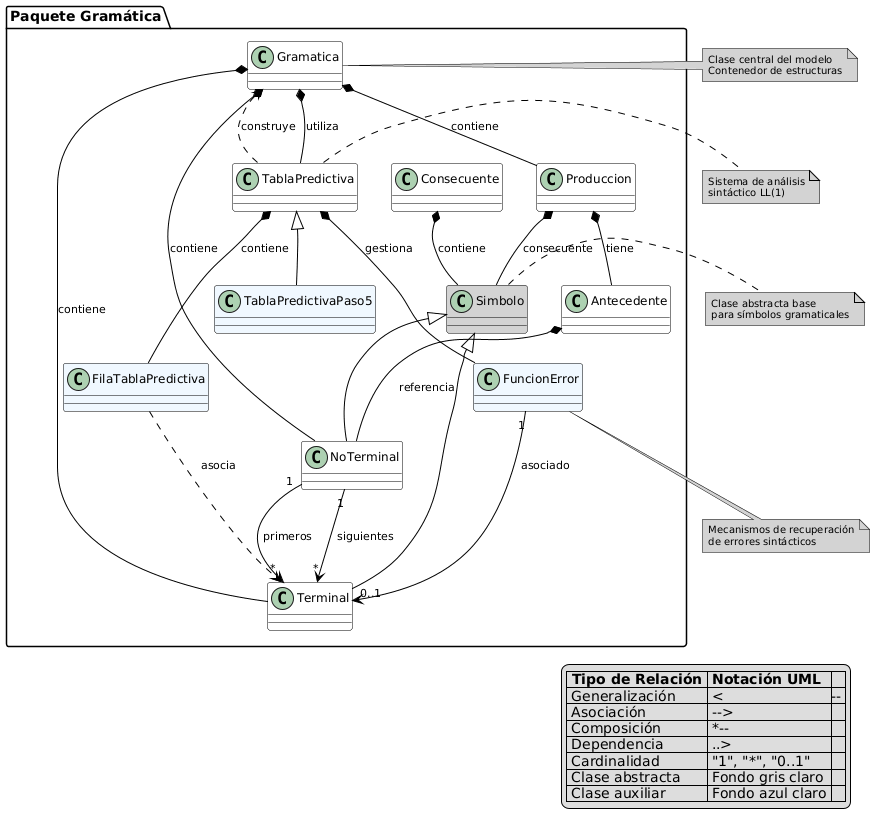
\includegraphics[width=0.9\textwidth]{figuras/Cap9/diagrama_gramatica_bueno.png}
    \caption{Diagrama de clases del paquete gramática - SimAS 3.0}
    \label{fig:diagrama_gramatica}
\end{figure}

\subsubsection{Patrones de diseño en el paquete gramática}

\begin{itemize}
    \item \textbf{Composite}: el patrón Composite se utiliza en la jerarquía de símbolos (Simbolo como componente abstracto, Terminal y NoTerminal como componentes concretos) \cite{gamma1995design}.
    \item \textbf{Observer/Observable}: implementado mediante JavaFX Properties para notificación automática de cambios en la UI cuando se modifican los datos del modelo \cite{gamma1995design}.
    \item \textbf{Strategy}: el patrón Strategy se utiliza en las funciones de error (FuncionError) que encapsulan diferentes estrategias de recuperación de errores \cite{gamma1995design}.
    \item \textbf{Factory Method}: implícito en los constructores de las clases que crean instancias con diferentes configuraciones iniciales \cite{gamma1995design}.
    \item \textbf{Singleton}: la clase Gramatica actúa como contenedor singleton para una gramática específica durante su edición \cite{gamma1995design}.
    \item \textbf{MVC (Model-View-Controller)}: el paquete completo sigue el patrón MVC donde las clases del paquete gramática representan el Modelo, las clases de vistas manejan la presentación, y los controladores coordinan la interacción \cite{burbeck1992applications}.
\end{itemize}

\subsection{Paquete utils}

El paquete \textbf{utils} contiene las clases de utilidad transversales que proporcionan funcionalidades comunes y servicios compartidos utilizados por todos los demás paquetes de SimAS 3.0. Este paquete implementa servicios transversales como gestión de pestañas, internacionalización, monitoreo de componentes y gestión de ventanas secundarias.

Las clases de este paquete permiten:
\begin{itemize}
    \item Gestión avanzada de pestañas y navegación entre ventanas
    \item Sistema completo de internacionalización con soporte multiidioma
    \item Monitoreo y supervisión automática de componentes de la interfaz
    \item Gestión de ventanas secundarias y comunicación entre ellas
    \item Utilidades comunes para todas las capas de la aplicación
\end{itemize}

\subsubsection{Clases del paquete utils}

Este paquete contiene 8 clases principales que proporcionan servicios transversales a toda la aplicación SimAS 3.0, organizadas por funcionalidad: gestión de pestañas, internacionalización, monitoreo y ventanas.

\subsubsection{Clase ActualizableTextos}

La clase \textbf{ActualizableTextos} es una interfaz que define el contrato para la actualización dinámica de textos en la interfaz de usuario cuando cambia el idioma de la aplicación.

\begin{longtable}[H]{|>{\columncolor[rgb]{0.63,0.79,0.95}}m{6cm} | m{8.5cm} |}
\caption{Clase ActualizableTextos - Interfaz de internacionalización}
\endfirsthead
\multicolumn{2}{c}{{\tablename\ \thetable{} -- continúa de la página anterior}} \\
\endhead
\hline \multicolumn{2}{|r|}{{Continúa en la página siguiente}} \\ \hline
\endfoot
\hline
\endlastfoot
\hline
\textbf{Nombre} & \textbf{ActualizableTextos} \\ \hline
\textbf{Descripción} & Interfaz que define el contrato para actualizar textos de la interfaz cuando cambia el idioma, implementada por todas las clases de UI que requieren internacionalización. \\ \hline
\textbf{Métodos} &
\begin{enumerate}
    \item \textbf{actualizarTextos(ResourceBundle)}: método que debe implementar cada clase para actualizar sus textos según el ResourceBundle proporcionado.
\end{enumerate}
\label{tabla_actualizable_textos}
\end{longtable}

\subsubsection{Clase LanguageItem}

La clase \textbf{LanguageItem} representa un elemento de idioma en el sistema de internacionalización, conteniendo información sobre el nombre del idioma, código de localización y bandera correspondiente.

\begin{longtable}[H]{|>{\columncolor[rgb]{0.63,0.79,0.95}}m{6cm} | m{8.5cm} |}
\caption{Clase LanguageItem - Elemento de idioma}
\endfirsthead
\multicolumn{2}{c}{{\tablename\ \thetable{} -- continúa de la página anterior}} \\
\endhead
\hline \multicolumn{2}{|r|}{{Continúa en la página siguiente}} \\ \hline
\endfoot
\hline
\endlastfoot
\hline
\textbf{Nombre} & \textbf{LanguageItem} \\ \hline
\textbf{Descripción} & Representa un idioma disponible en la aplicación, incluyendo su nombre, código de localización y bandera visual para el selector de idiomas. \\ \hline
\textbf{Atributos} &
\begin{enumerate}
    \item \textbf{name}: String con el nombre del idioma (ej: "Español", "English").
    \item \textbf{locale}: String con el código de localización (ej: "es", "en").
    \item \textbf{flagPath}: String con la ruta de la imagen de la bandera.
    \item \textbf{flagImageView}: ImageView que contiene la bandera visual del idioma.
\end{enumerate} \\ \hline
\textbf{Métodos} &
\begin{enumerate}
    \item \textbf{LanguageItem(String, String, String)}: constructor que inicializa el idioma con nombre, localización y ruta de bandera.
    \item \textbf{getName()}: obtiene el nombre del idioma.
    \item \textbf{getLocale()}: obtiene el código de localización.
    \item \textbf{getFlagPath()}: obtiene la ruta de la bandera.
    \item \textbf{getFlagImageView()}: obtiene el ImageView de la bandera.
    \item \textbf{toString()}: devuelve el nombre del idioma como representación textual.
    \item \textbf{equals(Object)}: compara dos LanguageItem por su código de localización.
    \item \textbf{hashCode()}: devuelve el hashCode basado en el código de localización.
\end{enumerate}
\label{tabla_language_item}
\end{longtable}

\subsubsection{Clase LanguageListCell}

La clase \textbf{LanguageListCell} es una celda personalizada para listas de selección de idiomas, que muestra la bandera y nombre del idioma de forma visual.

\begin{longtable}[H]{|>{\columncolor[rgb]{0.63,0.79,0.95}}m{6cm} | m{8.5cm} |}
\caption{Clase LanguageListCell - Celda de lista de idiomas}
\endfirsthead
\multicolumn{2}{c}{{\tablename\ \thetable{} -- continúa de la página anterior}} \\
\endhead
\hline \multicolumn{2}{|r|}{{Continúa en la página siguiente}} \\ \hline
\endfoot
\hline
\endlastfoot
\hline
\textbf{Nombre} & \textbf{LanguageListCell} \\ \hline
\textbf{Descripción} & Celda personalizada para ComboBox y ListView que muestra elementos de idioma con su bandera y nombre de forma visual. \\ \hline
\textbf{Atributos} &
\begin{enumerate}
    \item \textbf{Componentes FXML}: elementos de la interfaz para mostrar bandera y texto.
\end{enumerate} \\ \hline
\textbf{Métodos} &
\begin{enumerate}
    \item \textbf{LanguageListCell()}: constructor que inicializa la celda personalizada.
    \item \textbf{updateItem(LanguageItem, boolean)}: actualiza el contenido visual de la celda con el idioma correspondiente.
    \item \textbf{inicializarComponentes()}: configura los componentes visuales de la celda.
\end{enumerate}
\label{tabla_language_list_cell}
\end{longtable}

\subsubsection{Clase TabManager}

La clase \textbf{TabManager} es el gestor central de pestañas de la aplicación, responsable de crear, gestionar y coordinar todas las pestañas en múltiples ventanas.

\begin{longtable}[H]{|>{\columncolor[rgb]{0.63,0.79,0.95}}m{6cm} | m{8.5cm} |}
\caption{Clase TabManager - Gestor central de pestañas}
\endfirsthead
\multicolumn{2}{c}{{\tablename\ \thetable{} -- continúa de la página anterior}} \\
\endhead
\hline \multicolumn{2}{|r|}{{Continúa en la página siguiente}} \\ \hline
\endfoot
\hline
\endlastfoot
\hline
\textbf{Nombre} & \textbf{TabManager} \\ \hline
\textbf{Descripción} & Gestor central que maneja la creación, gestión y coordinación de todas las pestañas en la aplicación, incluyendo relaciones padre-hijo y grupos de gramáticas. \\ \hline
\textbf{Atributos} &
\begin{enumerate}
    \item \textbf{tabInstances}: Map que almacena instancias de pestañas por TabPane y tipo.
    \item \textbf{parentChildRelations}: Map que mantiene las relaciones padre-hijo entre pestañas.
    \item \textbf{elementoToGrupo}: Map que asocia elementos con sus grupos de gramática.
    \item \textbf{gruposGramatica}: Map que contiene los números de grupo para cada grupo.
    \item \textbf{resourceBundles}: Map que almacena ResourceBundles por TabPane.
    \item \textbf{contadorGrupos}: contador global para generar IDs únicos de grupo.
\end{enumerate} \\ \hline
\textbf{Métodos} &
\begin{enumerate}
    \item \textbf{getOrCreateTab(TabPane, Class, String, Object)}: obtiene o crea una pestaña del tipo especificado.
    \item \textbf{getOrCreateTab(TabPane, Class, String, Object, String, String)}: versión completa con IDs padre-hijo.
    \item \textbf{configurarMenuContextual(TabPane, ResourceBundle)}: configura el menú contextual de las pestañas.
    \item \textbf{reasignarNumerosGrupos(TabPane)}: reasigna números de grupo después de cambios.
    \item \textbf{crearGrupoGramatica(TabPane, String)}: crea un nuevo grupo de gramática.
    \item \textbf{setResourceBundle(TabPane, ResourceBundle)}: establece el ResourceBundle para un TabPane.
    \item \textbf{renumerarGrupos(TabPane)}: renumera todos los grupos de un TabPane.
    \item \textbf{limpiarRelacionesHuérfanas(TabPane)}: limpia relaciones padre-hijo huérfanas.
    \item \textbf{obtenerGruposActivos(TabPane)}: obtiene todos los grupos activos en un TabPane.
    \item \textbf{imprimirEstadoTabPane(TabPane)}: imprime el estado actual de un TabPane para debugging.
\end{enumerate}
\label{tabla_tab_manager}
\end{longtable}

\subsubsection{Clase TabPaneMonitor}

La clase \textbf{TabPaneMonitor} es un monitor singleton que supervisa continuamente el estado de todos los TabPane activos en la aplicación, validando consistencia y reparando automáticamente inconsistencias.

\begin{longtable}[H]{|>{\columncolor[rgb]{0.63,0.79,0.95}}m{6cm} | m{8.5cm} |}
\caption{Clase TabPaneMonitor - Monitor de pestañas}
\endfirsthead
\multicolumn{2}{c}{{\tablename\ \thetable{} -- continúa de la página anterior}} \\
\endhead
\hline \multicolumn{2}{|r|}{{Continúa en la página siguiente}} \\ \hline
\endfoot
\hline
\endlastfoot
\hline
\textbf{Nombre} & \textbf{TabPaneMonitor} \\ \hline
\textbf{Descripción} & Monitor singleton que supervisa continuamente todos los TabPanes activos, validando la consistencia de grupos y relaciones padre-hijo, y reparando automáticamente las inconsistencias detectadas. \\ \hline
\textbf{Atributos} &
\begin{enumerate}
    \item \textbf{instance}: instancia singleton del monitor.
    \item \textbf{monitoredTabPanes}: Map que contiene los TabPanes monitoreados.
    \item \textbf{scheduler}: ScheduledExecutorService para monitoreo periódico.
    \item \textbf{debugMode}: boolean que indica si está en modo debug.
    \item \textbf{movimientoEnProgreso}: boolean que indica si hay un movimiento en progreso.
    \item \textbf{contadorReparaciones}: Map que cuenta las reparaciones por TabPane.
\end{enumerate} \\ \hline
\textbf{Métodos} &
\begin{enumerate}
    \item \textbf{getInstance()}: obtiene la instancia singleton del monitor.
    \item \textbf{registrarTabPane(TabPane, String)}: registra un TabPane para monitoreo.
    \item \textbf{desregistrarTabPane(TabPane)}: desregistra un TabPane del monitoreo.
    \item \textbf{validarConsistenciaGlobal()}: valida la consistencia de todos los TabPanes monitoreados.
    \item \textbf{repararInconsistencias(TabPane, TabPaneInfo)}: repara inconsistencias detectadas.
    \item \textbf{obtenerEstadisticas()}: obtiene estadísticas del monitoreo.
    \item \textbf{setDebugMode(boolean)}: activa o desactiva el modo debug.
    \item \textbf{imprimirEstadoTabPane(TabPane)}: imprime el estado de un TabPane.
    \item \textbf{reiniciarContadores()}: reinicia los contadores de reparaciones.
\end{enumerate} \\ \hline
\textbf{Clase Interna TabPaneInfo} &
\begin{enumerate}
    \item \textbf{TabPaneInfo(TabPane, String)}: constructor de la información de TabPane.
    \item \textbf{tabPane}: referencia al TabPane monitoreado.
    \item \textbf{tabChangeListener}: listener para cambios en pestañas.
    \item \textbf{identifier}: identificador único del TabPane.
    \item \textbf{lastValidation}: timestamp de la última validación.
    \item \textbf{lastKnownGroups}: último estado conocido de grupos.
    \item \textbf{lastKnownRelations}: último estado conocido de relaciones.
\end{enumerate}
\label{tabla_tab_pane_monitor}
\end{longtable}

\subsubsection{Clase SecondaryWindow}

La clase \textbf{SecondaryWindow} extiende EditorWindow para crear ventanas secundarias que permiten trabajar con pestañas de forma independiente de la ventana principal.

\begin{longtable}[H]{|>{\columncolor[rgb]{0.63,0.79,0.95}}m{6cm} | m{8.5cm} |}
\caption{Clase SecondaryWindow - Ventanas secundarias}
\endfirsthead
\multicolumn{2}{c}{{\tablename\ \thetable{} -- continúa de la página anterior}} \\
\endhead
\hline \multicolumn{2}{|r|}{{Continúa en la página siguiente}} \\ \hline
\endfoot
\hline
\endlastfoot
\hline
\textbf{Nombre} & \textbf{SecondaryWindow} \\ \hline
\textbf{Descripción} & Extiende EditorWindow para crear ventanas secundarias que permiten trabajar con pestañas de forma independiente, facilitando la organización del espacio de trabajo. \\ \hline
\textbf{Atributos} &
\begin{enumerate}
    \item \textbf{activeWindows}: Map estático que mantiene todas las ventanas secundarias activas.
    \item \textbf{windowId}: identificador único de la ventana secundaria.
    \item \textbf{localTabPane}: TabPane específico de esta ventana secundaria.
    \item \textbf{stage}: Stage de la ventana secundaria.
    \item \textbf{bundle}: ResourceBundle para internacionalización.
    \item \textbf{windowNumber}: número secuencial de la ventana.
\end{enumerate} \\ \hline
\textbf{Métodos} &
\begin{enumerate}
    \item \textbf{SecondaryWindow(ResourceBundle, String)}: constructor que inicializa la ventana secundaria.
    \item \textbf{getActiveWindows()}: obtiene un mapa con todas las ventanas secundarias activas.
    \item \textbf{initialize()}: inicializa la ventana secundaria con sus componentes.
    \item \textbf{addTabFromDrag(Tab, String)}: añade una pestaña desde un arrastre.
    \item \textbf{setupDragAndDrop()}: configura las funcionalidades de arrastrar y soltar.
    \item \textbf{handleTabClose()}: maneja el cierre de pestañas en la ventana secundaria.
    \item \textbf{updateWindowTitle()}: actualiza el título de la ventana según su contenido.
    \item \textbf{closeWindow()}: cierra la ventana secundaria correctamente.
    \item \textbf{getWindowId()}: obtiene el identificador único de la ventana.
    \item \textbf{getStage()}: obtiene el Stage de la ventana secundaria.
    \item \textbf{getTabPane()}: obtiene el TabPane de la ventana secundaria.
\end{enumerate} \\ \hline
\textbf{Métodos Estáticos} &
\begin{enumerate}
    \item \textbf{getActiveWindows()}: obtiene todas las ventanas secundarias activas.
    \item \textbf{findWindowById(String)}: busca una ventana por su ID.
    \item \textbf{cleanupClosedWindows()}: limpia ventanas cerradas del registro.
\end{enumerate}
\label{tabla_secondary_window}
\end{longtable}

\subsubsection{Dependencias internas del paquete utils}

Las dependencias internas del paquete utils se ilustran en la Figura \ref{fig:diagrama_utils}, donde se puede apreciar la estructura organizada de servicios transversales que proporciona este paquete.

\begin{itemize}
    \item \textbf{TabManager $\leftrightarrow$ TabPaneMonitor}: TabManager utiliza TabPaneMonitor para supervisar los TabPane que gestiona.
    \item \textbf{SecondaryWindow $\rightarrow$ EditorWindow}: SecondaryWindow extiende EditorWindow para crear ventanas independientes.
    \item \textbf{SecondaryWindow $\rightarrow$ TabManager}: SecondaryWindow utiliza TabManager para gestionar sus pestañas.
    \item \textbf{LanguageItem $\leftrightarrow$ LanguageListCell}: LanguageListCell utiliza LanguageItem para mostrar idiomas en listas.
    \item \textbf{ActualizableTextos $\leftarrow$ (todas las clases de UI)}: interfaz implementada por todas las clases que requieren internacionalización.
    \item \textbf{TabManager $\leftrightarrow$ SecondaryWindow}: comunicación bidireccional para gestión de pestañas entre ventanas.
    \item \textbf{Archivos .properties}: todos los archivos de propiedades de idiomas son utilizados por el sistema de internacionalización.
\end{itemize}

\begin{figure}[H]
    \centering
    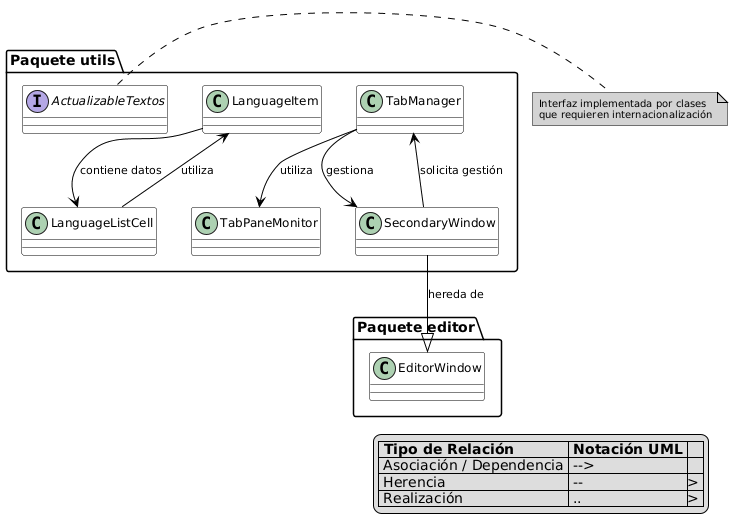
\includegraphics[width=0.9\textwidth]{figuras/Cap9/diagrama_utils.png}
    \caption{Diagrama de dependencias del paquete utils - SimAS 3.0}
    \label{fig:diagrama_utils}
\end{figure}

\subsubsection{Patrones de diseño en el paquete utils}

\begin{itemize}
    \item \textbf{Singleton}: implementado en TabPaneMonitor para asegurar una única instancia que supervise toda la aplicación \cite{gamma1995design}.
    \item \textbf{Observer}: utilizado en TabPaneMonitor para observar cambios en los TabPane y reaccionar automáticamente \cite{gamma1995design}.
    \item \textbf{Facade}: TabManager actúa como fachada que simplifica la gestión compleja de pestañas y relaciones \cite{gamma1995design}.
    \item \textbf{Factory Method}: implícito en los constructores de TabManager para crear diferentes tipos de pestañas \cite{gamma1995design}.
    \item \textbf{Monitor Object}: TabPaneMonitor implementa el patrón Monitor Object para sincronización segura de acceso a recursos compartidos.
    \item \textbf{Registry}: SecondaryWindow utiliza un registro estático para mantener todas las ventanas secundarias activas.
\end{itemize}

\subsection{Paquete editor}

El paquete \textbf{editor} contiene las clases responsables de la interfaz de usuario para la creación y edición de gramáticas de contexto libre en SimAS 3.0. Este paquete implementa el patrón de diseño MVC donde las clases del editor actúan como controladores que coordinan la interacción entre la vista (componentes JavaFX) y el modelo (paquete gramática).

Las clases de este paquete permiten:
\begin{itemize}
    \item Crear gramáticas mediante un asistente paso a paso
    \item Editar símbolos terminales y no terminales
    \item Gestionar producciones gramaticales
    \item Validar gramáticas creadas
    \item Gestionar múltiples editores en pestañas
    \item Integración completa con el sistema de internacionalización
\end{itemize}

\subsubsection{Clases del paquete editor}

Este paquete contiene 10 clases principales que conforman la interfaz de edición de SimAS 3.0, organizadas jerárquicamente desde la gestión de ventanas hasta los componentes específicos de edición.

\subsubsection{Clase EditorWindow}

La clase \textbf{EditorWindow} representa la ventana principal del editor de gramáticas, gestionando el ciclo de vida de la aplicación de edición y coordinando múltiples pestañas de edición.

\begin{longtable}[H]{|>{\columncolor[rgb]{0.63,0.79,0.95}}m{6cm} | m{8.5cm} |}
\caption{Clase EditorWindow - Ventana principal del editor}
\endfirsthead
\multicolumn{2}{c}{{\tablename\ \thetable{} -- continúa de la página anterior}} \\
\endhead
\hline \multicolumn{2}{|r|}{{Continúa en la página siguiente}} \\ \hline
\endfoot
\hline
\endlastfoot
\hline
\textbf{Nombre} & \textbf{EditorWindow} \\ \hline
\textbf{Descripción} & Gestiona la ventana principal del editor, incluyendo el sistema de pestañas, atajos de teclado y funcionalidades de arrastrar y soltar. \\ \hline
\textbf{Atributos} &
\begin{enumerate}
    \item \textbf{stage}: Stage principal de la ventana del editor.
    \item \textbf{tabPane}: TabPane que contiene todas las pestañas de edición.
    \item \textbf{bundle}: ResourceBundle para internacionalización.
\end{enumerate} \\ \hline
\textbf{Métodos} &
\begin{enumerate}
    \item \textbf{EditorWindow(ResourceBundle)}: constructor que inicializa la ventana con internacionalización.
    \item \textbf{initialize()}: configura la ventana, escena y componentes principales.
    \item \textbf{configurarAtajosTeclado(Scene)}: establece los atajos de teclado globales.
    \item \textbf{show()}: muestra la ventana del editor.
    \item \textbf{close()}: cierra la ventana del editor.
    \item \textbf{addEditorTab(String, Editor)}: añade una nueva pestaña de edición.
    \item \textbf{removeEditorTab(Editor)}: elimina una pestaña de edición.
\end{enumerate}
\label{tabla_editor_window}
\end{longtable}

\subsubsection{Clase Editor}

La clase \textbf{Editor} representa la interfaz principal de edición de una gramática específica, proporcionando acceso a todas las funcionalidades de edición y gestión.

\begin{longtable}[H]{|>{\columncolor[rgb]{0.63,0.79,0.95}}m{6cm} | m{8.5cm} |}
\caption{Clase Editor - Interfaz principal de edición}
\endfirsthead
\multicolumn{2}{c}{{\tablename\ \thetable{} -- continúa de la página anterior}} \\
\endhead
\hline \multicolumn{2}{|r|}{{Continúa en la página siguiente}} \\ \hline
\endfoot
\hline
\endlastfoot
\hline
\textbf{Nombre} & \textbf{Editor} \\ \hline
\textbf{Descripción} & Clase principal que representa un editor de gramáticas, gestionando la interfaz de usuario y la coordinación con el modelo de datos. \\ \hline
\textbf{Atributos} &
\begin{enumerate}
    \item \textbf{gramatica}: instancia de Gramatica que se está editando.
    \item \textbf{tabPane}: referencia al TabPane contenedor.
    \item \textbf{menuPane}: referencia al MenuPrincipal.
    \item \textbf{bundle}: ResourceBundle para internacionalización.
    \item \textbf{editorId}: identificador único del editor.
    \item \textbf{rootPane}: BorderPane raíz de la interfaz.
    \item \textbf{Componentes FXML}: botones, campos de texto, listas, etiquetas.
\end{enumerate} \\ \hline
\textbf{Métodos} &
\begin{enumerate}
    \item \textbf{Editor()}: constructor vacío para carga FXML.
    \item \textbf{Editor(TabPane, MenuPrincipal)}: constructor completo.
    \item \textbf{cargarFXML()}: carga la interfaz desde archivo FXML.
    \item \textbf{inicializarComponentes()}: configura todos los componentes de la UI.
    \item \textbf{configurarEventos()}: establece los manejadores de eventos.
    \item \textbf{actualizarListas()}: actualiza las listas de símbolos y producciones.
    \item \textbf{btnAnadir\_action()}: maneja la acción de añadir nueva gramática.
    \item \textbf{btnAbrir\_action()}: maneja la apertura de gramáticas existentes.
    \item \textbf{btnGuardar\_action()}: maneja el guardado de gramáticas.
    \item \textbf{btnEditar\_action()}: activa el modo de edición.
    \item \textbf{btnEliminar\_action()}: elimina la gramática actual.
    \item \textbf{btnValidar\_action()}: valida la gramática.
    \item \textbf{btnInforme\_action()}: genera informes de la gramática.
    \item \textbf{btnSimular\_action()}: inicia la simulación.
    \item \textbf{btnSalir\_action()}: cierra el editor.
    \item \textbf{actualizarTextos(ResourceBundle)}: actualiza textos para internacionalización.
\end{enumerate} \\ \hline
\textbf{Métodos} &
\begin{enumerate}
    \item \textbf{getGramatica()}: obtiene la gramática actual.
    \item \textbf{setGramatica(Gramatica)}: establece una nueva gramática.
    \item \textbf{getBundle()}: obtiene el ResourceBundle.
    \item \textbf{configurarRelacionesPadreHijo()}: configura el sistema de identificación.
    \item \textbf{crearGramatica()}: crea una nueva instancia de Gramatica.
\end{enumerate}
\label{tabla_editor}
\end{longtable}

\subsubsection{Clase PanelCreacionGramatica}

La clase \textbf{PanelCreacionGramatica} coordina el asistente de creación de gramáticas paso a paso, gestionando la navegación entre los diferentes pasos del proceso.

\begin{longtable}[H]{|>{\columncolor[rgb]{0.63,0.79,0.95}}m{6cm} | m{8.5cm} |}
\caption{Clase PanelCreacionGramatica - Asistente de creación}
\endfirsthead
\multicolumn{2}{c}{{\tablename\ \thetable{} -- continúa de la página anterior}} \\
\endhead
\hline \multicolumn{2}{|r|}{{Continúa en la página siguiente}} \\ \hline
\endfoot
\hline
\endlastfoot
\hline
\textbf{Nombre} & \textbf{PanelCreacionGramatica} \\ \hline
\textbf{Descripción} & Coordina el asistente paso a paso para la creación de gramáticas, gestionando la navegación y el flujo de datos entre los diferentes paneles. \\ \hline
\textbf{Atributos} &
\begin{enumerate}
    \item \textbf{tabPane}: TabPane contenedor de las pestañas.
    \item \textbf{paso1-4}: instancias de los paneles de cada paso del asistente.
    \item \textbf{panelPadre}: referencia al Editor padre.
    \item \textbf{menuPane}: referencia al MenuPrincipal.
    \item \textbf{gramaticaTemporal}: copia temporal de la gramática en edición.
    \item \textbf{bundle}: ResourceBundle para internacionalización.
    \item \textbf{creacionId}: identificador único del proceso de creación.
\end{enumerate} \\ \hline
\textbf{Métodos} &
\begin{enumerate}
    \item \textbf{PanelCreacionGramatica(Editor, TabPane, Gramatica, MenuPrincipal)}: constructor principal.
    \item \textbf{inicializarPaneles()}: inicializa todos los paneles del asistente.
    \item \textbf{configurarNavegacion()}: configura la navegación entre pasos.
    \item \textbf{validarPasoActual()}: valida el contenido del paso actual.
    \item \textbf{avanzarAlSiguientePaso()}: navega al siguiente paso del asistente.
    \item \textbf{retrocederAlPasoAnterior()}: navega al paso anterior.
    \item \textbf{finalizarCreacion()}: completa el proceso de creación.
    \item \textbf{cancelarCreacion()}: cancela el proceso de creación.
    \item \textbf{actualizarGramaticaTemporal()}: actualiza la gramática temporal con los datos actuales.
    \item \textbf{actualizarTextos(ResourceBundle)}: actualiza textos para internacionalización.
\end{enumerate}
\label{tabla_panel_creacion_gramatica}
\end{longtable}

\subsubsection{Clase PanelCreacionGramaticaPaso1}

La clase \textbf{PanelCreacionGramaticaPaso1} maneja el primer paso del asistente de creación, donde se definen los metadatos básicos de la gramática.

\begin{longtable}[H]{|>{\columncolor[rgb]{0.63,0.79,0.95}}m{6cm} | m{8.5cm} |}
\caption{Clase PanelCreacionGramaticaPaso1 - Paso 1: Metadatos}
\endfirsthead
\multicolumn{2}{c}{{\tablename\ \thetable{} -- continúa de la página anterior}} \\
\endhead
\hline \multicolumn{2}{|r|}{{Continúa en la página siguiente}} \\ \hline
\endfoot
\hline
\endlastfoot
\hline
\textbf{Nombre} & \textbf{PanelCreacionGramaticaPaso1} \\ \hline
\textbf{Descripción} & Primer paso del asistente de creación de gramáticas, donde se definen el nombre, descripción y símbolo inicial. \\ \hline
\textbf{Atributos} &
\begin{enumerate}
    \item \textbf{panelPadre}: referencia al PanelCreacionGramatica padre.
    \item \textbf{bundle}: ResourceBundle para internacionalización.
    \item \textbf{Componentes FXML}: campos de texto para nombre, descripción y símbolo inicial.
    \item \textbf{btnSiguiente}: botón para avanzar al siguiente paso.
    \item \textbf{btnCancelar}: botón para cancelar la creación.
\end{enumerate} \\ \hline
\textbf{Métodos} &
\begin{enumerate}
    \item \textbf{PanelCreacionGramaticaPaso1( PanelCreacionGramatica, ResourceBundle)}: constructor.
    \item \textbf{inicializarInterfaz()}: configura la interfaz del paso 1.
    \item \textbf{configurarValidacion()}: establece las reglas de validación.
    \item \textbf{setNombre(String)}: establece el nombre de la gramática.
    \item \textbf{setDescripcion(String)}: establece la descripción.
    \item \textbf{setSimboloInicial(String)}: establece el símbolo inicial.
    \item \textbf{validarCampos()}: valida que todos los campos requeridos estén completos.
    \item \textbf{btnSiguiente\_action()}: maneja el avance al siguiente paso.
    \item \textbf{btnCancelar\_action()}: maneja la cancelación.
    \item \textbf{actualizarTextos(ResourceBundle)}: actualiza textos para internacionalización.
\end{enumerate}
\label{tabla_panel_creacion_paso1}
\end{longtable}

\subsubsection{Clase PanelCreacionGramaticaPaso2}

La clase \textbf{PanelCreacionGramaticaPaso2} maneja el segundo paso del asistente de creación, donde se definen los símbolos terminales y no terminales.

\begin{longtable}[H]{|>{\columncolor[rgb]{0.63,0.79,0.95}}m{6cm} | m{8.5cm} |}
\caption{Clase PanelCreacionGramaticaPaso2 - Paso 2: Símbolos}
\endfirsthead
\multicolumn{2}{c}{{\tablename\ \thetable{} -- continúa de la página anterior}} \\
\endhead
\hline \multicolumn{2}{|r|}{{Continúa en la página siguiente}} \\ \hline
\endfoot
\hline
\endlastfoot
\hline
\textbf{Nombre} & \textbf{PanelCreacionGramaticaPaso2} \\ \hline
\textbf{Descripción} & Segundo paso del asistente donde se definen y gestionan los símbolos terminales y no terminales de la gramática. \\ \hline
\textbf{Atributos} &
\begin{enumerate}
    \item \textbf{panelPadre}: referencia al PanelCreacionGramatica padre.
    \item \textbf{menuPane}: referencia al MenuPrincipal.
    \item \textbf{tabPane}: TabPane para gestión de pestañas.
    \item \textbf{panelTerminales}: PanelSimbolosTerminales para gestión de terminales.
    \item \textbf{panelNoTerminales}: PanelSimbolosNoTerminales para gestión de no terminales.
    \item \textbf{bundle}: ResourceBundle para internacionalización.
    \item \textbf{btnSiguiente, btnAnterior, btnCancelar}: botones de navegación.
\end{enumerate} \\ \hline
\textbf{Métodos} &
\begin{enumerate}
    \item \textbf{PanelCreacionGramaticaPaso2( PanelCreacionGramatica, MenuPrincipal, TabPane)}: constructor.
    \item \textbf{inicializarPaneles()}: inicializa los paneles de símbolos.
    \item \textbf{configurarNavegacion()}: configura los botones de navegación.
    \item \textbf{validarSimbolos()}: valida que los símbolos definidos sean correctos.
    \item \textbf{asignarListaSimbolosTerminales( ObservableList<String>)}: asigna la lista de terminales.
    \item \textbf{asignarListaSimbolosNoTerminales( ObservableList<String>)}: asigna la lista de no terminales.
    \item \textbf{obtenerSimbolosTerminales()}: obtiene los símbolos terminales definidos.
    \item \textbf{obtenerSimbolosNoTerminales()}: obtiene los símbolos no terminales definidos.
    \item \textbf{btnSiguiente\_action()}: maneja el avance al siguiente paso.
    \item \textbf{btnAnterior\_action()}: maneja el retroceso al paso anterior.
    \item \textbf{btnCancelar\_action()}: maneja la cancelación.
    \item \textbf{actualizarTextos(ResourceBundle)}: actualiza textos para internacionalización.
\end{enumerate}
\label{tabla_panel_creacion_paso2}
\end{longtable}

\subsubsection{Clase PanelCreacionGramaticaPaso3}

La clase \textbf{PanelCreacionGramaticaPaso3} maneja el tercer paso del asistente, donde se definen las producciones de la gramática.

\begin{longtable}[H]{|>{\columncolor[rgb]{0.63,0.79,0.95}}m{6cm} | m{8.5cm} |}
\caption{Clase PanelCreacionGramaticaPaso3 - Paso 3: Producciones}
\endfirsthead
\multicolumn{2}{c}{{\tablename\ \thetable{} -- continúa de la página anterior}} \\
\endhead
\hline \multicolumn{2}{|r|}{{Continúa en la página siguiente}} \\ \hline
\endfoot
\hline
\endlastfoot
\hline
\textbf{Nombre} & \textbf{PanelCreacionGramaticaPaso3} \\ \hline
\textbf{Descripción} & Tercer paso del asistente donde se definen y gestionan las producciones de la gramática. \\ \hline
\textbf{Atributos} &
\begin{enumerate}
    \item \textbf{panelPadre}: referencia al PanelCreacionGramatica padre.
    \item \textbf{tabPane}: TabPane para gestión de pestañas.
    \item \textbf{menuPane}: referencia al MenuPrincipal.
    \item \textbf{panelProducciones}: PanelProducciones para gestión de producciones.
    \item \textbf{bundle}: ResourceBundle para internacionalización.
    \item \textbf{btnSiguiente, btnAnterior, btnCancelar}: botones de navegación.
\end{enumerate} \\ \hline
\textbf{Métodos} &
\begin{enumerate}
    \item \textbf{PanelCreacionGramaticaPaso3( PanelCreacionGramatica, TabPane, MenuPrincipal)}: constructor.
    \item \textbf{inicializarPanelProducciones()}: inicializa el panel de producciones.
    \item \textbf{configurarNavegacion()}: configura los botones de navegación.
    \item \textbf{validarProducciones()}: valida que las producciones definidas sean correctas.
    \item \textbf{asignarProducciones( ObservableList<Produccion>)}: asigna las producciones existentes.
    \item \textbf{obtenerProducciones()}: obtiene las producciones definidas.
    \item \textbf{btnSiguiente\_action()}: maneja el avance al siguiente paso.
    \item \textbf{btnAnterior\_action()}: maneja el retroceso al paso anterior.
    \item \textbf{btnCancelar\_action()}: maneja la cancelación.
    \item \textbf{actualizarTextos(ResourceBundle)}: actualiza textos para internacionalización.
\end{enumerate}
\label{tabla_panel_creacion_paso3}
\end{longtable}

\subsubsection{Clase PanelCreacionGramaticaPaso4}

La clase \textbf{PanelCreacionGramaticaPaso4} maneja el cuarto y último paso del asistente, donde se realiza la validación final y se completa la creación.

\begin{longtable}[H]{|>{\columncolor[rgb]{0.63,0.79,0.95}}m{6cm} | m{8.5cm} |}
\caption{Clase PanelCreacionGramaticaPaso4 - Paso 4: Validación}
\endfirsthead
\multicolumn{2}{c}{{\tablename\ \thetable{} -- continúa de la página anterior}} \\
\endhead
\hline \multicolumn{2}{|r|}{{Continúa en la página siguiente}} \\ \hline
\endfoot
\hline
\endlastfoot
\hline
\textbf{Nombre} & \textbf{PanelCreacionGramaticaPaso4} \\ \hline
\textbf{Descripción} & Cuarto y último paso del asistente donde se elige el símbolo inicial y se finaliza el proceso de creación. \\ \hline
\textbf{Atributos} &
\begin{enumerate}
    \item \textbf{panelPadre}: referencia al PanelCreacionGramatica padre.
    \item \textbf{tabPane}: TabPane para gestión de pestañas.
    \item \textbf{bundle}: ResourceBundle para internacionalización.
    \item \textbf{Componentes FXML}: etiquetas, botones de finalizar y cancelar.
    \item \textbf{areaValidacion}: área de texto para mostrar resultados de validación.
\end{enumerate} \\ \hline
\textbf{Métodos} &
\begin{enumerate}
    \item \textbf{PanelCreacionGramaticaPaso4( PanelCreacionGramatica, TabPane)}: constructor.
    \item \textbf{inicializarInterfaz()}: configura la interfaz del paso final.
    \item \textbf{realizarValidacionFinal()}: ejecuta todas las validaciones de la gramática.
    \item \textbf{mostrarResultadosValidacion()}: muestra los resultados de la validación.
    \item \textbf{btnFinalizar\_action()}: maneja la finalización exitosa del asistente.
    \item \textbf{btnVolver\_action()}: permite volver a pasos anteriores para correcciones.
    \item \textbf{btnCancelar\_action()}: maneja la cancelación completa.
    \item \textbf{generarResumenGramatica()}: genera un resumen de la gramática creada.
    \item \textbf{actualizarTextos(ResourceBundle)}: actualiza textos para internacionalización.
\end{enumerate}
\label{tabla_panel_creacion_paso4}
\end{longtable}

\subsubsection{Clase PanelProducciones}

La clase \textbf{PanelProducciones} proporciona la interfaz para editar y gestionar las producciones de la gramática.

\begin{longtable}[H]{|>{\columncolor[rgb]{0.63,0.79,0.95}}m{6cm} | m{8.5cm} |}
\caption{Clase PanelProducciones - Gestión de producciones}
\endfirsthead
\multicolumn{2}{c}{{\tablename\ \thetable{} -- continúa de la página anterior}} \\
\endhead
\hline \multicolumn{2}{|r|}{{Continúa en la página siguiente}} \\ \hline
\endfoot
\hline
\endlastfoot
\hline
\textbf{Nombre} & \textbf{PanelProducciones} \\ \hline
\textbf{Descripción} & Panel especializado para la creación, edición y eliminación de producciones gramaticales. \\ \hline
\textbf{Atributos} &
\begin{enumerate}
    \item \textbf{panelPadre}: referencia al PanelCreacionGramaticaPaso3 padre.
    \item \textbf{tabPane}: TabPane para gestión de pestañas.
    \item \textbf{producciones}: ObservableList de producciones.
    \item \textbf{noTerminales}: ObservableList de símbolos no terminales disponibles.
    \item \textbf{terminales}: ObservableList de símbolos terminales disponibles.
    \item \textbf{bundle}: ResourceBundle para internacionalización.
    \item \textbf{Componentes FXML}: ComboBox, TextField, ListViews, Buttons, Labels.
\end{enumerate} \\ \hline
\textbf{Métodos} &
\begin{enumerate}
    \item \textbf{PanelProducciones( PanelCreacionGramaticaPaso3, ObservableList<Produccion>, TabPane)}: constructor.
    \item \textbf{cargarFXML()}: carga la interfaz desde archivo FXML.
    \item \textbf{inicializarComponentes()}: configura todos los componentes de la UI.
    \item \textbf{configurarEventos()}: establece los manejadores de eventos.
    \item \textbf{actualizarListasSimbolos()}: actualiza las listas de símbolos disponibles.
    \item \textbf{btnInsertar\_action()}: inserta una nueva producción.
    \item \textbf{btnModificar\_action()}: modifica la producción seleccionada.
    \item \textbf{btnEliminar\_action()}: elimina la producción seleccionada.
    \item \textbf{btnBorrar\_action()}: borra el contenido del campo de consecuente.
    \item \textbf{btnEpsilon\_action()}: inserta el símbolo épsilon.
    \item \textbf{btnCancelar\_action()}: cancela la operación actual.
    \item \textbf{btnAceptar\_action()}: acepta y guarda los cambios.
    \item \textbf{validarProduccion()}: valida que la producción sea correcta.
    \item \textbf{actualizarTextos(ResourceBundle)}: actualiza textos para internacionalización.
\end{enumerate}
\label{tabla_panel_producciones}
\end{longtable}

\subsubsection{Clase PanelSimbolosTerminales}

La clase \textbf{PanelSimbolosTerminales} proporciona la interfaz para gestionar los símbolos terminales de la gramática.

\begin{longtable}[H]{|>{\columncolor[rgb]{0.63,0.79,0.95}}m{6cm} | m{8.5cm} |}
\caption{Clase PanelSimbolosTerminales - Gestión de terminales}
\endfirsthead
\multicolumn{2}{c}{{\tablename\ \thetable{} -- continúa de la página anterior}} \\
\endhead
\hline \multicolumn{2}{|r|}{{Continúa en la página siguiente}} \\ \hline
\endfoot
\hline
\endlastfoot
\hline
\textbf{Nombre} & \textbf{PanelSimbolosTerminales} \\ \hline
\textbf{Descripción} & Panel especializado para la gestión de símbolos terminales, incluyendo símbolos predefinidos y personalizados. \\ \hline
\textbf{Atributos} &
\begin{enumerate}
    \item \textbf{panelPadre}: referencia al PanelCreacionGramaticaPaso2 padre.
    \item \textbf{tabPane}: TabPane para gestión de pestañas.
    \item \textbf{simbolosTerminales}: ObservableList de símbolos terminales.
    \item \textbf{simbolosTemporales}: copia temporal de los símbolos.
    \item \textbf{simbolosSet}: Set para validación de unicidad.
    \item \textbf{bundle}: ResourceBundle para internacionalización.
    \item \textbf{simbolosPredefinidos}: array de símbolos comunes predefinidos.
    \item \textbf{Componentes FXML}: FlowPane, TextField, ListView, Buttons, Labels.
\end{enumerate} \\ \hline
\textbf{Métodos} &
\begin{enumerate}
    \item \textbf{PanelSimbolosTerminales( ObservableList<String>, TabPane, PanelCreacionGramaticaPaso2)}: constructor.
    \item \textbf{cargarFXML()}: carga la interfaz desde archivo FXML.
    \item \textbf{inicializarComponentes()}: configura todos los componentes de la UI.
    \item \textbf{crearBotonesPredefinidos()}: crea botones para símbolos predefinidos.
    \item \textbf{configurarEventos()}: establece los manejadores de eventos.
    \item \textbf{actualizarListaSimbolos()}: actualiza la lista visual de símbolos.
    \item \textbf{btnInsertar\_action()}: inserta un nuevo símbolo terminal.
    \item \textbf{btnModificar\_action()}: modifica el símbolo seleccionado.
    \item \textbf{btnEliminar\_action()}: elimina el símbolo seleccionado.
    \item \textbf{btnCancelar\_action()}: cancela la operación actual.
    \item \textbf{btnAceptar\_action()}: acepta y guarda los cambios.
    \item \textbf{validarSimbolo()}: valida que el símbolo sea único y válido.
    \item \textbf{actualizarTextos(ResourceBundle)}: actualiza textos para internacionalización.
\end{enumerate}
\label{tabla_panel_simbolos_terminales}
\end{longtable}

\subsubsection{Clase PanelSimbolosNoTerminales}

La clase \textbf{PanelSimbolosNoTerminales} proporciona la interfaz para gestionar los símbolos no terminales de la gramática.

\begin{longtable}[H]{|>{\columncolor[rgb]{0.63,0.79,0.95}}m{6cm} | m{8.5cm} |}
\caption{Clase PanelSimbolosNoTerminales - Gestión de no terminales}
\endfirsthead
\multicolumn{2}{c}{{\tablename\ \thetable{} -- continúa de la página anterior}} \\
\endhead
\hline \multicolumn{2}{|r|}{{Continúa en la página siguiente}} \\ \hline
\endfoot
\hline
\endlastfoot
\hline
\textbf{Nombre} & \textbf{PanelSimbolosNoTerminales} \\ \hline
\textbf{Descripción} & Panel especializado para la gestión de símbolos no terminales de la gramática. \\ \hline
\textbf{Atributos} &
\begin{enumerate}
    \item \textbf{panelPadre}: referencia al PanelCreacionGramaticaPaso2 padre.
    \item \textbf{tabPane}: TabPane para gestión de pestañas.
    \item \textbf{simbolosNoTerminales}: ObservableList de símbolos no terminales.
    \item \textbf{simbolosTemporales}: copia temporal de los símbolos.
    \item \textbf{simbolosSet}: Set para validación de unicidad.
    \item \textbf{bundle}: ResourceBundle para internacionalización.
    \item \textbf{Componentes FXML}: TextField, ListView, Buttons, Labels.
\end{enumerate} \\ \hline
\textbf{Métodos} &
\begin{enumerate}
    \item \textbf{PanelSimbolosNoTerminales( ObservableList<String>, TabPane, PanelCreacionGramaticaPaso2)}: constructor.
    \item \textbf{cargarFXML()}: carga la interfaz desde archivo FXML.
    \item \textbf{inicializarComponentes()}: configura todos los componentes de la UI.
    \item \textbf{configurarEventos()}: establece los manejadores de eventos.
    \item \textbf{actualizarListaSimbolos()}: actualiza la lista visual de símbolos.
    \item \textbf{btnInsertar\_action()}: inserta un nuevo símbolo no terminal.
    \item \textbf{btnModificar\_action()}: modifica el símbolo seleccionado.
    \item \textbf{btnEliminar\_action()}: elimina el símbolo seleccionado.
    \item \textbf{btnCancelar\_action()}: cancela la operación actual.
    \item \textbf{btnAceptar\_action()}: acepta y guarda los cambios.
    \item \textbf{validarSimbolo()}: valida que el símbolo sea único y válido.
    \item \textbf{actualizarTextos(ResourceBundle)}: actualiza textos para internacionalización.
\end{enumerate}
\label{tabla_panel_simbolos_no_terminales}
\end{longtable}

\subsubsection{Dependencias internas del paquete editor}

Las dependencias internas del paquete editor se ilustran en la Figura \ref{fig:diagrama_editor}, donde se puede apreciar la estructura jerárquica del asistente de creación y las relaciones entre los diferentes componentes de la interfaz.

\begin{itemize}
    \item \textbf{EditorWindow $\rightarrow$ Editor}: EditorWindow crea y gestiona múltiples instancias de Editor.
    \item \textbf{Editor $\rightarrow$ PanelCreacionGramatica}: Editor utiliza PanelCreacionGramatica para el asistente de creación.
    \item \textbf{PanelCreacionGramatica $\rightarrow$ PanelCreacionGramaticaPaso1-4}: PanelCreacionGramatica coordina los cuatro pasos del asistente.
    \item \textbf{PanelCreacionGramaticaPaso2 $\rightarrow$ PanelSimbolosTerminales, PanelSimbolosNoTerminales}: Paso 2 utiliza paneles específicos para gestión de símbolos.
    \item \textbf{PanelCreacionGramaticaPaso3 $\rightarrow$ PanelProducciones}: Paso 3 utiliza PanelProducciones para gestión de producciones.
    \item \textbf{PanelProducciones $\rightarrow$ gramatica.Gramatica}: PanelProducciones accede a la gramática para obtener símbolos disponibles.
    \item \textbf{PanelSimbolosTerminales $\rightarrow$ gramatica.Terminal}: PanelSimbolosTerminales gestiona símbolos terminales.
    \item \textbf{PanelSimbolosNoTerminales $\rightarrow$ gramatica.NoTerminal}: PanelSimbolosNoTerminales gestiona símbolos no terminales.
    \item \textbf{Todas las clases $\rightarrow$ utils.ActualizableTextos}: todas las clases del editor implementan esta interfaz para internacionalización.
    \item \textbf{Todas las clases $\rightarrow$ bienvenida.MenuPrincipal}: acceso al menú principal para navegación.
    \item \textbf{Todas las clases $\rightarrow$ utils.TabManager}: gestión de pestañas y grupos de gramáticas.
\end{itemize}

\subsubsection{Patrones de diseño en el paquete editor}

\begin{itemize}
    \item \textbf{MVC (Model-View-Controller)}: las clases del editor actúan como controladores coordinando entre las vistas JavaFX y el modelo gramática \cite{burbeck1992applications}.
    \item \textbf{Observer}: implementado mediante JavaFX Properties para notificación automática de cambios en la UI \cite{gamma1995design}.
    \item \textbf{Strategy}: los diferentes paneles (PanelProducciones, PanelSimbolosTerminales, etc.) implementan estrategias específicas de edición \cite{gamma1995design}.
    \item \textbf{Factory Method}: los constructores de las clases crean instancias con diferentes configuraciones iniciales \cite{gamma1995design}.
    \item \textbf{Composite}: la estructura jerárquica de paneles (PanelCreacionGramatica conteniendo PanelCreacionGramaticaPaso1-4) \cite{gamma1995design}.
    \item \textbf{Singleton}: uso implícito en la gestión de recursos compartidos como ResourceBundle \cite{gamma1995design}.
\end{itemize}

\begin{figure}[p]
    \centering
    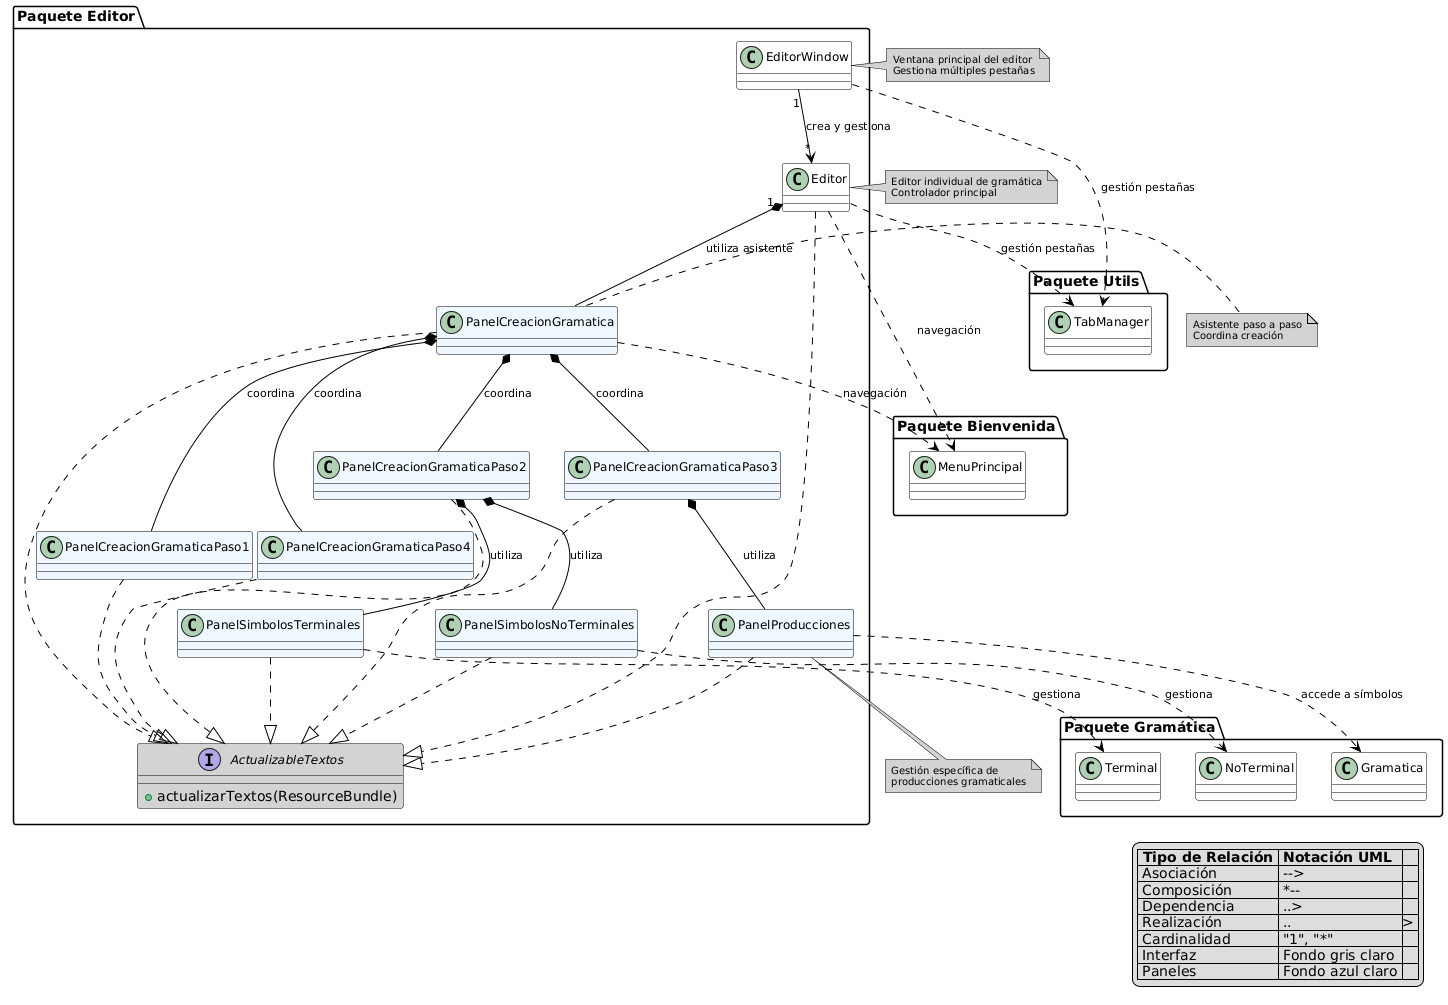
\includegraphics[angle=90,width=0.95\textwidth]{figuras/Cap9/diagrama_editor.png}
    \caption{Diagrama de clases del paquete editor - SimAS 3.0}
    \label{fig:diagrama_editor}
\end{figure}

\subsection{Paquete simulador}

El paquete \textbf{simulador} contiene las clases responsables de la simulación del análisis sintáctico descendente en SimAS 3.0. Este paquete implementa el núcleo funcional de la aplicación, permitiendo a los usuarios simular paso a paso el proceso de análisis sintáctico de cadenas de entrada utilizando gramáticas libres de contexto.

Las clases de este paquete permiten:
\begin{itemize}
    \item Simulación completa del análisis sintáctico descendente
    \item Visualización paso a paso del proceso de análisis
    \item Gestión de funciones de error y recuperación
    \item Creación y edición de cadenas de entrada
    \item Interfaz interactiva para la simulación
    \item Generación de informes y árboles de derivación
\end{itemize}

\subsubsection{Clases del paquete simulador}

Este paquete contiene 13 clases principales que implementan el sistema completo de simulación de análisis sintáctico, organizadas por funcionalidad: clases principales de simulación, pasos de la simulación descendente y componentes auxiliares.

\subsubsection{Clase PanelNuevaSimDescPaso}

La clase \textbf{PanelNuevaSimDescPaso} es una interfaz que define el contrato que deben implementar todos los pasos de la simulación descendente.

\begin{longtable}[H]{|>{\columncolor[rgb]{0.63,0.79,0.95}}m{6cm} | m{8.5cm} |}
\caption{Clase PanelNuevaSimDescPaso - Interfaz de pasos de simulación}
\endfirsthead
\multicolumn{2}{c}{{\tablename\ \thetable{} -- continúa de la página anterior}} \\
\endhead
\hline \multicolumn{2}{|r|}{{Continúa en la página siguiente}} \\ \hline
\endfoot
\hline
\endlastfoot
\hline
\textbf{Nombre} & \textbf{PanelNuevaSimDescPaso} \\ \hline
\textbf{Descripción} & Interfaz que define el contrato para todos los pasos de la simulación descendente, asegurando consistencia en la implementación. \\ \hline
\textbf{Métodos} &
\begin{enumerate}
    \item \textbf{getRoot()}: retorna el nodo raíz del paso de simulación.
\end{enumerate}
\label{tabla_panel_nueva_sim_desc_paso}
\end{longtable}

\subsubsection{Clase PanelNuevaSimDescPaso1}

La clase \textbf{PanelNuevaSimDescPaso1} implementa el primer paso de la simulación descendente, mostrando la gramática original y permitiendo la navegación entre pasos.

\begin{longtable}[H]{|>{\columncolor[rgb]{0.63,0.79,0.95}}m{6cm} | m{8.5cm} |}
\caption{Clase PanelNuevaSimDescPaso1 - Paso 1 de simulación}
\endfirsthead
\multicolumn{2}{c}{{\tablename\ \thetable{} -- continúa de la página anterior}} \\
\endhead
\hline \multicolumn{2}{|r|}{{Continúa en la página siguiente}} \\ \hline
\endfoot
\hline
\endlastfoot
\hline
\textbf{Nombre} & \textbf{PanelNuevaSimDescPaso1} \\ \hline
\textbf{Descripción} & Implementa el primer paso de la simulación descendente, mostrando la gramática original y permitiendo navegación entre los diferentes pasos del proceso. \\ \hline
\textbf{Atributos} &
\begin{enumerate}
    \item \textbf{panelPadre}: PanelSimuladorDesc que contiene este paso.
    \item \textbf{gramatica}: Gramatica que se está simulando.
    \item \textbf{bundle}: ResourceBundle para internacionalización.
    \item \textbf{root}: Parent que representa la interfaz gráfica del paso.
\end{enumerate} \\ \hline
\textbf{Métodos} &
\begin{enumerate}
    \item \textbf{PanelNuevaSimDescPaso1( PanelSimuladorDesc)}: constructor que inicializa el paso con su panel padre.
    \item \textbf{getRoot()}: retorna el nodo raíz de la interfaz gráfica.
    \item \textbf{actualizarTextos(ResourceBundle)}: actualiza los textos según el idioma seleccionado.
    \item \textbf{cargarFXML()}: carga el archivo FXML correspondiente al paso.
    \item \textbf{inicializarBotones()}: configura los botones de navegación.
\end{enumerate}
\label{tabla_panel_nueva_sim_desc_paso1}
\end{longtable}

\subsubsection{Clase PanelNuevaSimDescPaso2}

La clase \textbf{PanelNuevaSimDescPaso2} implementa el segundo paso de la simulación descendente, mostrando los símbolos terminales y no terminales.

\begin{longtable}[H]{|>{\columncolor[rgb]{0.63,0.79,0.95}}m{6cm} | m{8.5cm} |}
\caption{Clase PanelNuevaSimDescPaso2 - Paso 2 de simulación}
\endfirsthead
\multicolumn{2}{c}{{\tablename\ \thetable{} -- continúa de la página anterior}} \\
\endhead
\hline \multicolumn{2}{|r|}{{Continúa en la página siguiente}} \\ \hline
\endfoot
\hline
\endlastfoot
\hline
\textbf{Nombre} & \textbf{PanelNuevaSimDescPaso2} \\ \hline
\textbf{Descripción} & Implementa el segundo paso de la simulación descendente, mostrando los símbolos terminales y no terminales de la gramática. \\ \hline
\textbf{Atributos} &
\begin{enumerate}
    \item \textbf{panelPadre}: PanelSimuladorDesc que contiene este paso.
    \item \textbf{gramatica}: Gramatica que se está simulando.
    \item \textbf{bundle}: ResourceBundle para internacionalización.
    \item \textbf{root}: Parent que representa la interfaz gráfica del paso.
\end{enumerate} \\ \hline
\textbf{Métodos} &
\begin{enumerate}
    \item \textbf{PanelNuevaSimDescPaso2( PanelSimuladorDesc)}: constructor que inicializa el paso con su panel padre.
    \item \textbf{getRoot()}: retorna el nodo raíz de la interfaz gráfica.
    \item \textbf{actualizarTextos(ResourceBundle)}: actualiza los textos según el idioma seleccionado.
\end{enumerate}
\label{tabla_panel_nueva_sim_desc_paso2}
\end{longtable}

\subsubsection{Clase PanelNuevaSimDescPaso3}

La clase \textbf{PanelNuevaSimDescPaso3} implementa el tercer paso de la simulación descendente, mostrando los conjuntos First y Follow.

\begin{longtable}[H]{|>{\columncolor[rgb]{0.63,0.79,0.95}}m{6cm} | m{8.5cm} |}
\caption{Clase PanelNuevaSimDescPaso3 - Paso 3 de simulación}
\endfirsthead
\multicolumn{2}{c}{{\tablename\ \thetable{} -- continúa de la página anterior}} \\
\endhead
\hline \multicolumn{2}{|r|}{{Continúa en la página siguiente}} \\ \hline
\endfoot
\hline
\endlastfoot
\hline
\textbf{Nombre} & \textbf{PanelNuevaSimDescPaso3} \\ \hline
\textbf{Descripción} & Implementa el tercer paso de la simulación descendente, mostrando los conjuntos First y Follow de los símbolos no terminales. \\ \hline
\textbf{Atributos} &
\begin{enumerate}
    \item \textbf{panelPadre}: PanelSimuladorDesc que contiene este paso.
    \item \textbf{gramatica}: Gramatica que se está simulando.
    \item \textbf{bundle}: ResourceBundle para internacionalización.
    \item \textbf{root}: Parent que representa la interfaz gráfica del paso.
\end{enumerate} \\ \hline
\textbf{Métodos} &
\begin{enumerate}
    \item \textbf{PanelNuevaSimDescPaso3( PanelSimuladorDesc)}: constructor que inicializa el paso con su panel padre.
    \item \textbf{getRoot()}: retorna el nodo raíz de la interfaz gráfica.
    \item \textbf{actualizarTextos(ResourceBundle)}: actualiza los textos según el idioma seleccionado.
\end{enumerate}
\label{tabla_panel_nueva_sim_desc_paso3}
\end{longtable}

\subsubsection{Clase PanelNuevaSimDescPaso4}

La clase \textbf{PanelNuevaSimDescPaso4} implementa el cuarto paso de la simulación descendente, mostrando la tabla predictiva.

\begin{longtable}[H]{|>{\columncolor[rgb]{0.63,0.79,0.95}}m{6cm} | m{8.5cm} |}
\caption{Clase PanelNuevaSimDescPaso4 - Paso 4 de simulación}
\endfirsthead
\multicolumn{2}{c}{{\tablename\ \thetable{} -- continúa de la página anterior}} \\
\endhead
\hline \multicolumn{2}{|r|}{{Continúa en la página siguiente}} \\ \hline
\endfoot
\hline
\endlastfoot
\hline
\textbf{Nombre} & \textbf{PanelNuevaSimDescPaso4} \\ \hline
\textbf{Descripción} & Implementa el cuarto paso de la simulación descendente, mostrando la tabla predictiva completa con sus celdas y funciones de error. \\ \hline
\textbf{Atributos} &
\begin{enumerate}
    \item \textbf{panelPadre}: PanelSimuladorDesc que contiene este paso.
    \item \textbf{gramatica}: Gramatica que se está simulando.
    \item \textbf{bundle}: ResourceBundle para internacionalización.
    \item \textbf{root}: Parent que representa la interfaz gráfica del paso.
\end{enumerate} \\ \hline
\textbf{Métodos} &
\begin{enumerate}
    \item \textbf{PanelNuevaSimDescPaso4( PanelSimuladorDesc)}: constructor que inicializa el paso con su panel padre.
    \item \textbf{getRoot()}: retorna el nodo raíz de la interfaz gráfica.
    \item \textbf{actualizarTextos(ResourceBundle)}: actualiza los textos según el idioma seleccionado.
\end{enumerate}
\label{tabla_panel_nueva_sim_desc_paso4}
\end{longtable}

\subsubsection{Clase PanelNuevaSimDescPaso5}

La clase \textbf{PanelNuevaSimDescPaso5} implementa el quinto paso de la simulación descendente, permitiendo la edición de funciones de error.

\begin{longtable}[H]{|>{\columncolor[rgb]{0.63,0.79,0.95}}m{6cm} | m{8.5cm} |}
\caption{Clase PanelNuevaSimDescPaso5 - Paso 5 de simulación}
\endfirsthead
\multicolumn{2}{c}{{\tablename\ \thetable{} -- continúa de la página anterior}} \\
\endhead
\hline \multicolumn{2}{|r|}{{Continúa en la página siguiente}} \\ \hline
\endfoot
\hline
\endlastfoot
\hline
\textbf{Nombre} & \textbf{PanelNuevaSimDescPaso5} \\ \hline
\textbf{Descripción} & Implementa el quinto paso de la simulación descendente, permitiendo la edición y configuración de funciones de error para recuperación de errores. \\ \hline
\textbf{Atributos} &
\begin{enumerate}
    \item \textbf{panelPadre}: PanelSimuladorDesc que contiene este paso.
    \item \textbf{gramatica}: Gramatica que se está simulando.
    \item \textbf{bundle}: ResourceBundle para internacionalización.
    \item \textbf{root}: Parent que representa la interfaz gráfica del paso.
\end{enumerate} \\ \hline
\textbf{Métodos} &
\begin{enumerate}
    \item \textbf{PanelNuevaSimDescPaso5( PanelSimuladorDesc)}: constructor que inicializa el paso con su panel padre.
    \item \textbf{getRoot()}: retorna el nodo raíz de la interfaz gráfica.
    \item \textbf{actualizarTextos(ResourceBundle)}: actualiza los textos según el idioma seleccionado.
\end{enumerate}
\label{tabla_panel_nueva_sim_desc_paso5}
\end{longtable}

\subsubsection{Clase PanelNuevaSimDescPaso6}

La clase \textbf{PanelNuevaSimDescPaso6} implementa el sexto y último paso de la simulación descendente, que corresponde al \textbf{Simulador} principal donde se ejecuta la simulación completa del análisis sintáctico.

\begin{longtable}[H]{|>{\columncolor[rgb]{0.63,0.79,0.95}}m{6cm} | m{8.5cm} |}
\caption{Clase PanelNuevaSimDescPaso6 - Paso 6 (Simulador) de simulación}
\endfirsthead
\multicolumn{2}{c}{{\tablename\ \thetable{} -- continúa de la página anterior}} \\
\endhead
\hline \multicolumn{2}{|r|}{{Continúa en la página siguiente}} \\ \hline
\endfoot
\hline
\endlastfoot
\hline
\textbf{Nombre} & \textbf{ PanelNuevaSimDescPaso6} \\ \hline
\textbf{Descripción} & Implementa el sexto y último paso de la simulación descendente (el Simulador principal), permitiendo ejecutar la simulación completa del análisis sintáctico. \\ \hline
\textbf{Atributos} &
\begin{enumerate}
    \item \textbf{panelPadre}: PanelSimuladorDesc que contiene este paso.
    \item \textbf{gramatica}: Gramatica que se está simulando.
    \item \textbf{bundle}: ResourceBundle para internacionalización.
    \item \textbf{root}: Parent que representa la interfaz gráfica del paso.
\end{enumerate} \\ \hline
\textbf{Métodos} &
\begin{enumerate}
    \item \textbf{PanelNuevaSimDescPaso6(PanelSimuladorDesc)}: constructor que inicializa el paso con su panel padre.
    \item \textbf{getRoot()}: retorna el nodo raíz de la interfaz gráfica.
    \item \textbf{actualizarTextos(ResourceBundle)}: actualiza los textos según el idioma seleccionado.
\end{enumerate}
\label{tabla_panel_nueva_sim_desc_paso6}
\end{longtable}

\subsubsection{Clase PanelSimuladorDesc}

La clase \textbf{PanelSimuladorDesc} es el controlador principal para la simulación descendente, coordinando todos los pasos del proceso de análisis sintáctico.

\begin{longtable}[H]{|>{\columncolor[rgb]{0.63,0.79,0.95}}m{6cm} | m{8.5cm} |}
\caption{Clase PanelSimuladorDesc - Controlador principal de simulación}
\endfirsthead
\multicolumn{2}{c}{{\tablename\ \thetable{} -- continúa de la página anterior}} \\
\endhead
\hline \multicolumn{2}{|r|}{{Continúa en la página siguiente}} \\ \hline
\endfoot
\hline
\endlastfoot
\hline
\textbf{Nombre} & \textbf{PanelSimuladorDesc} \\ \hline
\textbf{Descripción} & Controlador principal que coordina toda la simulación descendente, gestionando los diferentes pasos, la gramática y la interacción con el usuario. \\ \hline
\textbf{Atributos} &
\begin{enumerate}
    \item \textbf{tabPane}: TabPane donde se muestran los pasos de simulación.
    \item \textbf{gramatica}: Gramatica que se está simulando.
    \item \textbf{gramaticaOriginal}: copia independiente de la gramática original.
    \item \textbf{pasoActual}: número del paso actual en la simulación.
    \item \textbf{pasos}: ArrayList con todos los pasos de la simulación.
    \item \textbf{bundle}: ResourceBundle para internacionalización.
    \item \textbf{tablaPredictivaExtendidaGlobal}: TablaPredictivaPaso5 con funciones de error.
    \item \textbf{simuladorId}: identificador único del simulador.
    \item \textbf{simuladoresActivos}: Map estático con todos los simuladores activos.
\end{enumerate} \\ \hline
\textbf{Métodos} &
\begin{enumerate}
    \item \textbf{PanelSimuladorDesc(Gramatica, TabPane, ResourceBundle)}: constructor principal.
    \item \textbf{PanelSimuladorDesc(Gramatica, TabPane, ResourceBundle, String)}: constructor con ID personalizado.
    \item \textbf{configurarRelacionesPadreHijo()}: configura las relaciones entre pestañas.
    \item \textbf{inicializarTablaPredictivaYFuncionesError()}: inicializa la tabla predictiva y funciones de error.
    \item \textbf{crearPestanaSimulacion()}: crea la pestaña principal de simulación.
    \item \textbf{mostrarPaso(int)}: muestra un paso específico de la simulación.
    \item \textbf{getBundle()}: obtiene el ResourceBundle actual.
    \item \textbf{getTablaPredictivaExtendidaGlobal()}: obtiene la tabla predictiva extendida.
\end{enumerate}
\label{tabla_panel_simulador_desc}
\end{longtable}

\subsubsection{Clase PanelSimulacion}

La clase \textbf{PanelSimulacion} implementa un panel completo para la simulación interactiva del análisis sintáctico.

\begin{longtable}[H]{|>{\columncolor[rgb]{0.63,0.79,0.95}}m{6cm} | m{8.5cm} |}
\caption{Clase PanelSimulacion - Panel de simulación interactiva}
\endfirsthead
\multicolumn{2}{c}{{\tablename\ \thetable{} -- continúa de la página anterior}} \\
\endhead
\hline \multicolumn{2}{|r|}{{Continúa en la página siguiente}} \\ \hline
\endfoot
\hline
\endlastfoot
\hline
\textbf{Nombre} & \textbf{PanelSimulacion} \\ \hline
\textbf{Descripción} & Panel que proporciona una interfaz completa para la simulación interactiva del análisis sintáctico, permitiendo controlar paso a paso el proceso de análisis. \\ \hline
\textbf{Atributos} &
\begin{enumerate}
    \item \textbf{gramatica}: Gramatica que se está simulando.
    \item \textbf{tablaPredictiva}: TablaPredictivaPaso5 con funciones de error.
    \item \textbf{funcionesError}: List de FuncionError disponibles.
    \item \textbf{entrada}: String que representa la cadena de entrada.
    \item \textbf{pila}: Stack que simula la pila del analizador.
    \item \textbf{entradaActual}: List que contiene los símbolos de entrada.
    \item \textbf{posicionEntrada}: posición actual en la cadena de entrada.
    \item \textbf{simulacionEnCurso}: boolean que indica si la simulación está activa.
    \item \textbf{bundle}: ResourceBundle para internacionalización.
\end{enumerate} \\ \hline
\textbf{Métodos} &
\begin{enumerate}
    \item \textbf{PanelSimulacion(Gramatica, ResourceBundle)}: constructor que inicializa el panel de simulación.
    \item \textbf{inicializarComponentes()}: configura todos los componentes de la interfaz.
    \item \textbf{simular()}: ejecuta un paso de la simulación.
    \item \textbf{reiniciar()}: reinicia la simulación al estado inicial.
    \item \textbf{actualizarInterfaz()}: actualiza la interfaz gráfica según el estado actual.
    \item \textbf{procesarEntrada(String)}: procesa la cadena de entrada para análisis.
\end{enumerate}
\label{tabla_panel_simulacion}
\end{longtable}

\subsubsection{Clase SimulacionFinal}

La clase \textbf{SimulacionFinal} implementa la simulación completa del análisis sintáctico con capacidades avanzadas de visualización y control.

\begin{longtable}[H]{|>{\columncolor[rgb]{0.63,0.79,0.95}}m{6cm} | m{8.5cm} |}
\caption{Clase SimulacionFinal - Simulación completa avanzada}
\endfirsthead
\multicolumn{2}{c}{{\tablename\ \thetable{} -- continúa de la página anterior}} \\
\endhead
\hline \multicolumn{2}{|r|}{{Continúa en la página siguiente}} \\ \hline
\endfoot
\hline
\endlastfoot
\hline
\textbf{Nombre} & \textbf{SimulacionFinal} \\ \hline
\textbf{Descripción} & Implementa la simulación completa del análisis sintáctico con capacidades avanzadas como historial, navegación, generación de informes y visualización de árboles de derivación. \\ \hline
\textbf{Atributos} &
\begin{enumerate}
    \item \textbf{gramatica}: Gramatica que se está simulando.
    \item \textbf{tablaPredictiva}: TablaPredictivaPaso5 con funciones de error.
    \item \textbf{funcionesError}: List de FuncionError para recuperación.
    \item \textbf{pila}: Stack que simula la pila del analizador.
    \item \textbf{entradaActual}: ArrayList con la cadena de entrada.
    \item \textbf{historialPasos}: ObservableList con el historial de pasos.
    \item \textbf{pasoActual}: posición actual en la simulación.
    \item \textbf{bundle}: ResourceBundle para internacionalización.
\end{enumerate} \\ \hline
\textbf{Métodos} &
\begin{enumerate}
    \item \textbf{SimulacionFinal(Gramatica, ResourceBundle)}: constructor principal.
    \item \textbf{inicializarComponentes()}: configura la interfaz gráfica completa.
    \item \textbf{simularPaso()}: ejecuta un paso individual de la simulación.
    \item \textbf{simularCompleta()}: ejecuta toda la simulación automáticamente.
    \item \textbf{retrocederPaso()}: retrocede un paso en la simulación.
    \item \textbf{reiniciarSimulacion()}: reinicia la simulación al estado inicial.
    \item \textbf{generarInforme()}: genera un informe completo de la simulación.
    \item \textbf{mostrarArbolDerivacion()}: muestra el árbol de derivación.
    \item \textbf{actualizarTextos(ResourceBundle)}: actualiza textos según el idioma.
\end{enumerate}
\label{tabla_simulacion_final}
\end{longtable}

\subsubsection{Clase PanelGramaticaOriginal}

La clase \textbf{PanelGramaticaOriginal} muestra la gramática original en una pestaña separada con soporte para internacionalización.

\begin{longtable}[H]{|>{\columncolor[rgb]{0.63,0.79,0.95}}m{6cm} | m{8.5cm} |}
\caption{Clase PanelGramaticaOriginal - Panel de gramática original}
\endfirsthead
\multicolumn{2}{c}{{\tablename\ \thetable{} -- continúa de la página anterior}} \\
\endhead
\hline \multicolumn{2}{|r|}{{Continúa en la página siguiente}} \\ \hline
\endfoot
\hline
\endlastfoot
\hline
\textbf{Nombre} & \textbf{PanelGramaticaOriginal} \\ \hline
\textbf{Descripción} & Panel que muestra la gramática original en una pestaña separada, permitiendo visualizar todas las producciones de forma clara y organizada. \\ \hline
\textbf{Atributos} &
\begin{enumerate}
    \item \textbf{gramaticaOriginal}: Gramatica original que se muestra.
    \item \textbf{bundle}: ResourceBundle para internacionalización.
\end{enumerate} \\ \hline
\textbf{Métodos} &
\begin{enumerate}
    \item \textbf{PanelGramaticaOriginal(Gramatica, ResourceBundle)}: constructor que inicializa el panel.
    \item \textbf{actualizarTextos(ResourceBundle)}: actualiza los textos según el idioma seleccionado.
\end{enumerate}
\label{tabla_panel_gramatica_original}
\end{longtable}

\subsubsection{Clase NuevaFuncionError}

La clase \textbf{NuevaFuncionError} permite crear y configurar nuevas funciones de error para la recuperación en el análisis sintáctico.

\begin{longtable}[H]{|>{\columncolor[rgb]{0.63,0.79,0.95}}m{6cm} | m{8.5cm} |}
\caption{Clase NuevaFuncionError - Creación de funciones de error}
\endfirsthead
\multicolumn{2}{c}{{\tablename\ \thetable{} -- continúa de la página anterior}} \\
\endhead
\hline \multicolumn{2}{|r|}{{Continúa en la página siguiente}} \\ \hline
\endfoot
\hline
\endlastfoot
\hline
\textbf{Nombre} & \textbf{NuevaFuncionError} \\ \hline
\textbf{Descripción} & Permite crear y configurar nuevas funciones de error para la recuperación automática durante el análisis sintáctico descendente. \\ \hline
\textbf{Atributos} &
\begin{enumerate}
    \item \textbf{gramatica}: Gramatica donde se aplicarán las funciones de error.
    \item \textbf{paso4}: PanelNuevaSimDescPaso4 que contiene este componente.
    \item \textbf{bundle}: ResourceBundle para internacionalización.
    \item \textbf{root}: Parent que representa la interfaz gráfica.
\end{enumerate} \\ \hline
\textbf{Métodos} &
\begin{enumerate}
    \item \textbf{NuevaFuncionError(Gramatica, PanelNuevaSimDescPaso4, ResourceBundle)}: constructor principal.
    \item \textbf{inicializarCampos()}: configura los campos de entrada para la función de error.
    \item \textbf{crearFuncionError()}: crea una nueva función de error con los parámetros especificados.
    \item \textbf{actualizarTextos(ResourceBundle)}: actualiza los textos según el idioma seleccionado.
\end{enumerate}
\label{tabla_nueva_funcion_error}
\end{longtable}

\subsubsection{Clase EditorCadenaEntradaController}

La clase \textbf{EditorCadenaEntradaController} proporciona una interfaz para editar y gestionar las cadenas de entrada que se utilizarán en la simulación.

\begin{longtable}[H]{|>{\columncolor[rgb]{0.63,0.79,0.95}}m{6cm} | m{8.5cm} |}
\caption{Clase EditorCadenaEntradaController - Editor de cadenas de entrada}
\endfirsthead
\multicolumn{2}{c}{{\tablename\ \thetable{} -- continúa de la página anterior}} \\
\endhead
\hline \multicolumn{2}{|r|}{{Continúa en la página siguiente}} \\ \hline
\endfoot
\hline
\endlastfoot
\hline
\textbf{Nombre} & \textbf{EditorCadenaEntradaController} \\ \hline
\textbf{Descripción} & Controlador que proporciona una interfaz completa para editar, validar y gestionar las cadenas de entrada que se utilizarán en las simulaciones de análisis sintáctico. \\ \hline
\textbf{Atributos} &
\begin{enumerate}
    \item \textbf{cadenaActual}: String que contiene la cadena de entrada actual.
    \item \textbf{gramatica}: Gramatica utilizada para validar la cadena.
    \item \textbf{bundle}: ResourceBundle para internacionalización.
\end{enumerate} \\ \hline
\textbf{Métodos} &
\begin{enumerate}
    \item \textbf{validarCadena(String)}: valida que la cadena sea aceptada por la gramática.
    \item \textbf{editarCadena()}: abre el editor para modificar la cadena de entrada.
    \item \textbf{guardarCadena(String)}: guarda la cadena editada.
    \item \textbf{actualizarTextos(ResourceBundle)}: actualiza los textos según el idioma seleccionado.
\end{enumerate}
\label{tabla_editor_cadena_entrada_controller}
\end{longtable}

\subsubsection{Dependencias internas del paquete simulador}

Las dependencias internas del paquete simulador se ilustran en la Figura \ref{fig:diagrama_simulador}, donde se puede apreciar la estructura organizada del sistema de simulación paso a paso y sus interacciones con otros paquetes.

\begin{itemize}
    \item \textbf{PanelSimuladorDesc $\rightarrow$ PanelNuevaSimDescPaso1-6}: PanelSimuladorDesc contiene y coordina todos los pasos de simulación, siendo PanelNuevaSimDescPaso6 el Simulador principal.
    \item \textbf{PanelNuevaSimDescPaso1-6 $\rightarrow$ PanelNuevaSimDescPaso}: todos los pasos implementan la interfaz PanelNuevaSimDescPaso.
    \item \textbf{PanelSimuladorDesc $\leftrightarrow$ Gramatica}: utiliza la gramática para la simulación.
    \item \textbf{PanelSimuladorDesc $\leftrightarrow$ TablaPredictivaPaso5}: utiliza la tabla predictiva extendida.
    \item \textbf{SimulacionFinal $\rightarrow$ Gramatica}: utiliza la gramática para simulación completa.
    \item \textbf{PanelSimulacion $\rightarrow$ TablaPredictivaPaso5}: utiliza la tabla predictiva para simulación interactiva.
    \item \textbf{NuevaFuncionError $\rightarrow$ PanelNuevaSimDescPaso4}: se integra en el paso 4 de la simulación.
    \item \textbf{PanelGramaticaOriginal $\rightarrow$ Gramatica}: muestra la gramática original.
    \item \textbf{EditorCadenaEntradaController $\rightarrow$ Gramatica}: valida cadenas contra la gramática.
    \item \textbf{Todas las clases $\rightarrow$ ResourceBundle}: utilizan internacionalización.
\end{itemize}

\begin{figure}[p]
    \centering
    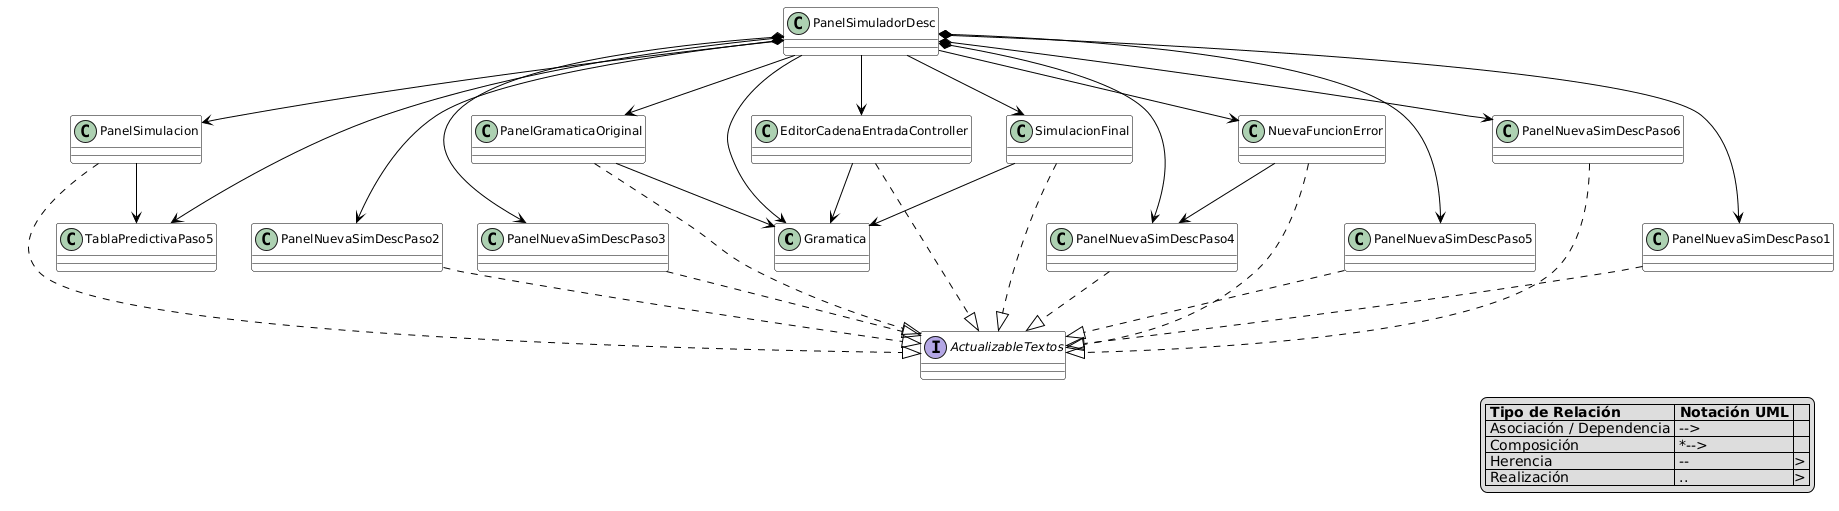
\includegraphics[angle=90,width=\textwidth,height=\textheight]{figuras/Cap9/diagrama_simulador2.png}
    \caption{Diagrama de dependencias del paquete simulador - SimAS 3.0}
    \label{fig:diagrama_simulador}
\end{figure}

\subsubsection{Patrones de diseño en el paquete simulador}

\begin{itemize}
    \item \textbf{MVC (Model-View-Controller)}: el paquete sigue el patrón MVC donde las clases del paquete gramática son el Modelo, las clases del simulador son los Controladores, y los componentes FXML son las Vistas \cite{burbeck1992applications}.
    \item \textbf{Strategy}: los diferentes pasos de simulación (PanelNuevaSimDescPaso1-6) implementan estrategias diferentes para cada fase del análisis \cite{gamma1995design}.
    \item \textbf{Observer}: las clases implementan ActualizableTextos para observar cambios en el idioma y actualizar automáticamente la interfaz \cite{gamma1995design}.
    \item \textbf{Factory Method}: los constructores de PanelSimuladorDesc crean diferentes configuraciones de simuladores según los parámetros \cite{gamma1995design}.
    \item \textbf{Registry}: PanelSimuladorDesc mantiene un registro estático de todos los simuladores activos para gestión centralizada.
\end{itemize}
